\documentclass[sigconf, nonacm]{acmart}
 

\newtheorem{definition}{Definition}
\newcommand{\eat}[1]{}

\usepackage{algorithm2e}

\RestyleAlgo{ruled}

\usepackage{multirow}


\setcopyright{acmcopyright}
\acmYear{2022}
\acmDOI{10.1145/1122445.1122456}

%% These commands are for a PROCEEDINGS abstract or paper.
%%\acmConference[Woodstock '18]{Woodstock '18: ACM Symposium on Neural
%%  Gaze Detection}{June 03--05, 2018}{Woodstock, NY}
%%\acmBooktitle{Woodstock '18: ACM Symposium on Neural Gaze Detection,
%%  June 03--05, 2018, Woodstock, NY}
%%\acmPrice{15.00}
%%\acmISBN{978-1-4503-XXXX-X/18/06}


%%
%% Submission ID.
%% Use this when submitting an article to a sponsored event. You'll
%% receive a unique submission ID from the organizers
%% of the event, and this ID should be used as the parameter to this command.
%%\acmSubmissionID{123-A56-BU3}

%%
%% The majority of ACM publications use numbered citations and
%% references.  The command \citestyle{authoryear} switches to the
%% "author year" style.
%%
%% If you are preparing content for an event
%% sponsored by ACM SIGGRAPH, you must use the "author year" style of
%% citations and references.
%% Uncommenting
%% the next command will enable that style.
%%\citestyle{acmauthoryear}




%%
%% end of the preamble, start of the body of the document source.
\begin{document}

%%
%% The "title" command has an optional parameter,
%% allowing the author to define a "short title" to be used in page headers.
\title{Evaluating Dataset portions based on query logs}

%%
%% The "author" command and its associated commands are used to define
%% the authors and their affiliations.
%% Of note is the shared affiliation of the first two authors, and the
%% "authornote" and "authornotemark" commands
%% used to denote shared contribution to the research.

\author{Leonardo Vicentini}
\affiliation{%
  \country{232221}}
\email{leonardo.vicentini@studenti.unitn.it}

\author{Luca Vian}
\affiliation{%
  \country{238744}
}
\email{luca.vian@studenti.unitn.it}



%%
%% By default, the full list of authors will be used in the page
%% headers. Often, this list is too long, and will overlap
%% other information printed in the page headers. This command allows
%% the author to define a more concise list
%% of authors' names for this purpose.

%%
%% This command processes the author and affiliation and title
%% information and builds the first part of the formatted document.
\settopmatter{printacmref=false}
\maketitle

\section{Introduction}
%\label{sec:context}

We live in a world in which the amount of digital information that surrounds us is so high that we need to use some recommendation systems everyday in order to filter the ones that could be interesting for us. We need to use these technologies so frequently that we almost take for granted their presence in all the devices and platforms that we use during our days.\cite{commons-Importance}

A \textbf{Recommendation System} is a tool that is able to filter and prioritize the relevant information for users, based on their personalized basis. This process allows to reduce the information load that the user will receive after having learnt, in an implicit and explicit way, their preferences.\cite{Raghuwanshi-Intro} The functionalities provided by a well-developed recommendation system could be helpful both for the platform that host it, because it will increase in traffic, and for the users, that will be more satisfied.\cite{Ilyas-Intro}

Many businesses' revenues are directly related to the quality of their recommendation system. For example, search engines like Google are interested in proposing web pages that could be found meaningful by the users. Other services instead, like Amazon and AirBnB, are interested in proposing products and apartments based on the users' preferences. Finally, other services, such as Netflix and Spotify, propose a well-developed recommendation system in order to have a competitive platform useful for growing a large user base.

\subsection{Netflix}
Netflix, indeed, represent one of the most successful examples of recommendation systems: its movies are proposed by considering some \textbf{attributes} that they have (like information about the titles, such as their genre, categories, actors, release year, etc) together with the \textbf{habits that a certain user has} (the time of the day when a user accesses the service, the average length of his/her stay in the platform, and so on). The preferences of an user are obtained both in a directed way, for example by understanding what the users like using their ratings or requesting some feedback, either in a non-directed way, analyzing the users' habits.\cite{Netflix-Recommendation} 

The data that Netflix's recommendation system uses are very different, and as a result, they must be treated and processed differently: there are data that can change or stay the same over time, that can be discrete or continuous, and that can be known or unknown. Typically, the unknown and unfixed information pertains to the users.

\subsection{Challenges behind a recommendation system}
As illustrated, the development of a recommendation system could be very challenging for many reasons independently by its scope and scenario. The key problems are related to the lack of data collection and to the fact that both the information fields that could be considered relevant, as well as their values, may change over time.\cite{Macmanus-5Problems} Furthermore, how to use those data at disposition is quite complex and not intuitive, so only a few companies can provide a very high level of user satisfaction with their recommendation systems.

To those difficulties another one is added, which is related to dealing with those information in an \textbf{efficient} and feasible manner, not obtainable with na\"ive approaches. 

It should be noted that there are no issues with cold starts in the scenario under consideration: cases where new items or users are added  are not within the scope of the problem addressed by this work.

\subsection{Approaches to tackle this task}
Throughout the years, research has focused on the complications associated with the recommendation task in order to find the best approaches and techniques for dealing with it. The main ones can be divided into three major categories:
\begin{itemize}
  \item Content-based systems
  \item Collaborative filtering systems
  \item Hybrid recommendations approaches
\end{itemize}
Each category is characterized by their own main advantages such that, depending on the specific task that must be performed, we can prefer a specific approach with respect to another one.

Content-based systems focus on \textbf{properties} of items. Similarity of items is determined by measuring the similarity in their properties.\cite{Book-ch9}
In general, collaborative filtering systems focus instead on the \textbf{relationship} between users and items. For instance, the similarity of two items could be determined by the similarity of the ratings of those items by the users who have rated both of them.\cite{Book-ch9}

Usually some preliminary steps are required to avoid either slow run-time computation and results that are far from the actual preferences of the  users. Similarity, for instance, could be used to \textbf{cluster} users and/or items into small groups with high similarity. 


Most recommendation systems now employ a \textbf{hybrid approach} that combines collaborative filtering, content-based filtering, and other techniques. Hybrid approaches can be implemented in several ways, including separately making content-based and collaborative-filtering predictions and then combining them; adding content-based capabilities to a collaborative filtering approach (and vice versa); and unifying the approaches into a single model. \cite{hybrid-intro}

\subsection{Our query recommendation system}
The context on which we decided to focus on is similar to the Netflix one, even if we have decided to put more emphasis in recommending some queries related to a set of movies instead of recommending the movies themselves. In other words, we wanted to compute how much a set of queries identifying one or more movies characterized by \textbf{discrete} and \textbf{continuous} attributes could satisfy a user's preferences. The most effective approach we were able to obtain was composed of two different Collaborative Filtering components weighted according to \textbf{query result cardinality}.


Our tool's ultimate goal is to be able to complete the tasks outlined in section \ref{sec:problem_statement} regardless of the domain being analyzed. In other words, if "MOVIES" is the current domain, "SUPERMARKET PRODUCTS" could be an alternative one. To be able to perform the later formalized tasks correctly regardless of the domain chosen, the tool or set of algorithms must be elastic and make as few assumptions as possible. 


\section{Problem Statement}
\label{sec:problem_statement}

We can define the previously mentioned problem more formally, specifically by dividing our task into \textbf{two major sub-tasks} or \textbf{sub-problems}.

For the first sub-task, the inputs given are:
\begin{itemize}

  \item A \textbf{relational table} $RT$: where each item $i$ is represented by a row containing 
  some values that characterize specific attributes of that item. Therefore, each row represent a tuple of the shape: $\langle attr1, attr2, attr3, ..., attrN \rangle$. All the fields of all the tuples have a value and there are no NULL values. Formally: 
  $$\mathbf{RT} = \left{ \left(v_{1,i}, v_{2,i}, \dots, v_{N,i} \right) \mid v_{j,i} \in \mathbf{V} \right}$$

    
  \item A \textbf{user set} $US$: 
  where each user $u$ is represented by one row that contains only the id of the user $u$. Formally:
  $$\mathbf{US} = \left{ u_i \mid u_i \in \mathbf{U_{ID}} \right}$$
    
  \item A \textbf{query set} $QS$: where each query $q$ previously posed is represented by a row.
  Each row starts with an identifier of the query and continues with its definition composed by conjunction of \emph{"attribute=value"} conditions. For the same query, there couldn't be more than a condition regarding the same attribute. Formally: $$\mathbf{QS} = \left{ \left(q_i, \left{ \left(a_j, v_j \right) \right}_{j=1}^n \right) \mid q_i \in \mathbf{Q_{ID}}, \left(a_j, v_j \right) \in \mathbf{AV}, n \ge 1 \right}$$

  \item A \textbf{utility matrix} $U$: a matrix in which each row corresponds to a user $u$, each column to a query $q$ and for some user-query pairs $(u,q)$, a satisfaction rating between 0 and 100 is provided. 
  So, $U_{u,q}$ represents the satisfaction rating for user $u$ and query $q$ and the condition $ 0 \le U_{u,q} \le 100 $ holds. Formally: 
$$
\begin{aligned}
N &= |\mathbf{US}| \\
M &= |\mathbf{QS}| \\
\mathbf{R} &= \left\{ r \in \mathbb{R} \mid 0 \leq r \leq 100 \right\} \\
\mathbf{U} &= \left\{ \mathbf{U}_{u,q} \in \mathbf{R} \cup {\text\{{NULL\}}} \mid 0 \leq u < N, 0 \leq q < M \right\} 
\end{aligned}
$$

\end{itemize}





The goal of the first task is to \textbf{fill} the utility matrix's user-query pairs that still don't have a value in a coherent way with the interest of each user. In this manner we could, given that completed matrix $C$ and a user $u$, return the top-k queries that might be of interest to a specific user $u$.
More formally, the outputs of the first task are:
\begin{itemize}
    \item A \textbf{completed utility matrix} $C$, where $C_{u,q}$ represents the satisfaction rating for user $u$ and query $q$, including the previously missing values. Formally:
    $$
\mathbf{C} &= \left\{ \mathbf{C}_{u,q} \in \mathbf{R} \mid 0 \leq u < N, 0 \leq q < M \right\} 
$$
with $R$, $N$ and $M$ defined like in the case of $U$.
    \item A \textbf{list of top-$k$ queries} $L$ that might be of interest to a specific user $u$.
    Formally:
    $$
    \begin{aligned}
        \mathbf{L} &= { \left(u, q_i, r_{i} \right) \mid u \in \mathbf{US}, q_i \in \mathbf{QS}, r_{i} \in \mathbf{R},1 \leq i \leq k, 
    \end{aligned}    
    $$    
    $$
    \begin{aligned}
 
        \forall x, y \in \{1, 2, 3, ..., k\}, x < y, 100 \geq r_x \geq r_y  \geq \mathbf{BR} \geq 0
        }
    \end{aligned}    
    $$    
    
where $r_{i}$ represents the satisfaction rating for the fixed user $u$ and query $q_{i}$, $R$ defined as before. We define the set of good ratings $GR$ = \{$r_1, r_2, ..., r_k$\} and bad ratings $BR$ such that $\mathbf{GR} \cap \mathbf{BR} = \varnothing$ holds. \\
\end{itemize}


After completing the first sub-task, we want to \textbf{broaden} the problem in a more general sense: given the elements produced by the previous task as input, we want to find a way to compute a utility matrix for a query in general for all the users. 

More formally, the output of the second sub-task is:
\begin{itemize}
    \item An \textbf{array} $QU$ of satisfaction ratings which represents the utility of a query in general, (i.e. \textbf{an unseen query}) for all the users in the user set $US$. Formally:
$$
\begin{aligned}
\mathbf{QU} &= \left{ \left( q, u_i, r_i \right) \mid q \in \mathbf{NQS}, u_i \in \mathbf{US}, r_{i} \in \mathbf{R}, 0 \leq i < N \right} 
\end{aligned}
$$

where $NQS$ is a set of unseen queries (i.e.: $\mathbf{NQS} \cap \mathbf{QS} = \varnothing$), $r_{i}$ represents the satisfaction rating for user $u_{i}$ and the fixed query $q$, $R$ and $N$ are defined as before.

\end{itemize}



\subsection{Our scenario}

The inputs and the outputs managed by the tool are organized in \textbf{csv} files.

The context that we exploited in order to create a tool for accomplishing the previously formalized task is related to movies. 

In the context of this specific chosen domain, the tuples composing the relation table $RT$ are of the shape: $\langle name, genre, runtime, year, \\country, score \rangle$.
Note that \textit{rating} could represent a generic rating given by a review aggregator like Rotten Tomatoes or IMDb.
\\

As a result, the relational table contains some discrete fields (such as genre and nationality) as well as some continuous ones (such as length, publication year, and rating) that are also used in the defined queries. We also assumed that users could have an unspoken preference for the genre, nationality, length, and publication year when generating the partial utility matrix, while there are fields that have no significance (the title) and others that influence the preferences of all users in the same way (the rating).
\section{Related work}
\label{sec:related_work}
\subsection{Utility Matrix and Complete Utility Matrix}
The concept of \textbf{Utility Matrix} is fundamental in order to understand the problem statement and also the solution proposed. An Utility Matrix is a matrix composed of $u$ rows, with $u$ the number of \textbf{users} considered, and $i$ columns, with $i$ the number of \textbf{items} belonging to the Relational Table taken into account. In the interception between a certain row $n$ and a certain column $m$ there could be a value, to represent the preference score given by the user $n$ for the item $m$, or not, in the case the user $n$ still have not expressed explicitly a rating regarding the item $m$.\cite{Book-ch9} The main goal of a recommendation system regards filling the missing values of this Utility Matrix in order to obtain a complete one, in which the \textbf{blank ratings} are deduced in a coherent way by the ones explicitly expressed in the partial one. 

\subsection{Collaborative filtering systems}
\subsubsection{Item-Item Collaborative filtering systems}
The \textbf{collaborative filtering systems}, and in particular the \textbf{item-item} collaborative filtering ones, represent the first approach tried in developing the proposed solution and that ended up being an important part of it. Indeed, it was demonstrated that the item-item collaborative filtering approaches represent one of the most valid methods because they work referring to the items' attributes that are much simpler in comparison to the ones that regards the users, that instead can be characterized by multiple tastes.\cite{Book-ch9} The main idea of this approach, that will be better developed during the \textbf{Chapter \ref{sec:solution}}, is related in finding, for each item, a certain set of a chosen cardinality composed by its most similar ones. In this way, it's possible to assume that an \textbf{unrated cell} belonging to the utility matrix will have a rating obtained by combining the known ratings of other similar items in a weighted way \cite{Book-ch9}.
Also the theory regarding the advantages and disadvantages of a Collaborative Filtering System suggested why it would work well in a context like ours. Indeed:
\begin{itemize}
    \item The main advantages regards its ability to be used \textbf{independently} by the nature and the attributes' shape. This aspect is critical in developing a solution that will work well regardless of the dataset proposed.
    \item The common disadvantages of a collaborative filtering system, for example the Cold Start (the inability of identifying the taste of some users due to the lack of their ratings) and the one related, similarly, to the fact that a newly introduced item will not have any valuation, will not regard our scenario. Those problems indeed often characterize  \textbf{online contexts}, in which new data are presented over time to the system.
\end{itemize}
\subsubsection{Why a bigger dataset can be helpful in solving our task}
The fact that the ratings computation consists in finding the items that are similar to one chosen has a consequence that more will be the data in a dataset, better will be the results found. This works because:
\begin{itemize}
    \item more are the \textbf{items} considered, more probable will be to have, in the dataset, a set of items very similar to any one proposed.
    \item more are the \textbf{users} considered, more will be the number of ratings given by them to the items. This situation is also advantageous in order to find groups of similar items.
    \item also a \textbf{less sparse} utility matrix will be helpful in order to fill it in a better way. Indeed, also in this case, a greater number of known ratings will be helpful in order to understand better the items features, useful to find precisely the more similar items to one chosen.
\end{itemize}
\subsubsection{Approaches to reduce the time complexity}
Even if having more data will be helpful in computing a more coherent complete utility matrix, this will also have the \textbf{drawback} of analyzing and filling a greater matrix at the expenses of the performance in time. For this reason, some approaches were developed in order to fill an utility matrix with a lower complexity, having as consequence a slightly worse ratings predictions. 
The main approach used regards the \textbf{clustering}, with which is reduced the number of users, of items or of both by considering together the users or the items that are similar between them. This clustering procedure is performed by establishing a distance measure between the users and the items based on the ratings that regards them and, if their distance is under a threshold, it is possible to cluster them and consider them as elements having the same behavior. After having filled the clustered utility matrix, it is possible to expand it by assigning, to each user or item belonging to the same cluster, the rating regarding the cluster itself.
\subsection{Hybrid recommendation approaches}
A recommendation system that combines the predictions made by different ones is known as a \textbf{hybrid recommendation system}. Those approaches are quite popular and used due to the fact that usually it is hard to find a single recommender model that will fit well a given dataset. The solution proposed (Chapter \ref{sec:solution}) use one of the most popular methods for developing a hybrid recommendation system, which is combining, in a \textbf{weighted way}, the prediction performed by two or more different recommendation systems.


\subsection{Distances}
\label{sec:distances}

When creating a recommendation system, different distance measures of similarity can be used in a variety of situations. 

\subsubsection{Cosine similarity}

$$
S_c(A, B):= cos(\theta) = \frac{A\cdot B}{\left \| A \right \|\left \| B \right \|} =\frac{\sum_{i=1}^{n}A_iB_i}{\sqrt{\sum_{i=1}^{n}A_i^{2}}\sqrt{\sum_{i=1}^{n}B_i^{2}}}
$$
\textbf{Cosine similarity} is a measure of similarity between two sequences of numbers (vectors).

\subsubsection{Centered cosine similarity}
Referring to cosine similarity, if the attribute vectors are normalized by subtracting the vector means (e.g., $A - \bar{A}$ ), the measure is called the Centered cosine similarity and is equivalent to the \textbf{Pearson correlation coefficient}.

\subsubsection{Jaccard similarity}

The Jaccard index, also known as the \textbf{Jaccard similarity} coefficient, is a statistic used for gauging the similarity and diversity of sample sets. \cite{Jaccard}

$$
J(A,B) = \frac{\left |A \cap B  \right |}{\left |  A \cup B\right |} = \frac{\left | A \cap B   \right | }{\left | A \right | + \left | B  \right | -\left | A \cap B \right |}
$$


\subsection{Programming language and libraries}
The entire solution was developed in \textbf{Python}. Mainly, the Pandas, NumPy and Scikit-learn.metrics libraries were leveraged.



%CHECK:
%https://assets.amazon.science/76/9e/7eac89c14a838746e91dde0a5e9f/two-decades-of-recommender-systems-at-amazon.pdf

%https://cseweb.ucsd.edu//classes/fa17/cse291-b/reading/Amazon-Recommendations.pdf




\section{Solution}
\label{sec:solution}

The path leading to the final solution was guided by analysis of related topics, reasoning deemed logical, and empirical results.

The proposed solution is a \textbf{hybrid recommendation system} leveraging a linear combination of \textbf{Expanded-Item-Item Collaborative Filtering} and \textbf{Compact Item-Item Collaborative Filtering} based on \textbf{query result cardinality}.


Therefore, the solution consists of 3 main components:
\begin{itemize}
    \item Compact (Standard) Item-Item Collaborative Filtering component
    \item Expanded-Item-Item Collaborative Filtering component
    \item Hybridization component
\end{itemize}


The first 2 components are used to obtain 2 \textit{Complete Utility Matrices}, which are \textbf{combined} according to a precise logic (i.e., using the cardinality of the result set of each query).

In the current configuration, the following logic is enforced: if a query's cardinality is high, a greater weight is given to the rating provided by the utility matrix of the compact method; instead, if the cardinality is low, a greater weight is given to the rating provided by the utility matrix of the expanded method.
The basic reasoning behind this was the fact that if a query is composed only by few items as result, it is possible to get the queries' ratings from the ones of their results. When, instead, the rating computation regards a query having an higher number of results, the prediction couldn't be computed correctly by starting from the one of its items. This because, summing up together a great number of predictions, each one characterized by a small inaccuracy, will have end up in a result in which all those errors are accumulated. 


In the \textbf{Compact Item-Item} Collaborative Filtering component, the queries were treated \textbf{directly} as items, whereas in the \textbf{Expanded Item-Item} Collaborative Filtering component, items are relational table tuples.


Since the solution devised an offline setting an important assumption were made: \textbf{heavy pre-computation task} are tolerated. This assumption was fundamental in order to keep our solution valid because of the fact that the intermediate user-item utility matrix, that will be computed and filled in the expanded collaborative filtering approach, has a numbers of cells much higher in comparison to the utility matrix representing the main input of the problem statement.
The intermediate results computed, i.e., compact complete utility matrix and expanded complete utility matrix are saved into ".csv" format which are then exploited to execute the two tasks.





\subsection{Compact Item-Item Collaborative Filtering component}
\label{sec:compact-item-item-cf-solution}
The Compact Item-Item Collaborative Filtering component was the first one to be developed since it would have been used as starting point for the Expanded version. 
Moreover, this component is used, as is, as part of the final solution.
The core part of this component is an implementation of a \textbf{standard} Collaborative Filtering algorithm. 
In this Compact version, items are the queries previously posed.

The \textbf{task} to be performed by this component is the generation of a \textit{Complete Utility Matrix} starting from the \textit{Utility Matrix} as input and filling it with newly calculated ratings where ratings were previously unknown.
As a validation proof, the implementation was tested during the development on a small dummy dataset.

To break down the implementation of the previously described algorithm, four major phases can be identified:
\begin{itemize}
    \item Pre-processing
    \item Computing similarities between items
    \item Calculating the ratings
    \item Generating the \textit{Complete Utility Matrix}
\end{itemize}


\subsubsection{Pre-processing}
The \textbf{input} that this component leverages is the only \textit{Utility Matrix} which is stored in a \verb+.csv+ file.
Each row $u$ represents a user, each column $q$ represents a query and each cell ($u$,$q$) represents a rating $r$ given by the user $u$ for the query $q$. If the user $u$ has not expressed his rating for the query $q$, the corresponding cell is empty. 

Once parsed from file, the \textit{Utility Matrix} is transposed and the missing values are replaced with $NaN$s. We should point out the fact that the transposition was made just to be able to verify that the actual implementation was correct, the operations that will be later described are symmetrically equivalent with respect to rows and columns.

A \textit{Centered Matrix}  is generated from the Transposed Utility Matrix as follows: if the cell contains a valid rating (not $NaN$), the Centered Matrix cell value is the rating minus row mean (which represent the mean rating of the relative query).

Instead, the cells of the \textit{Centered Matrix} containing \textit{NaN} values are filled with the mean of the query ratings (the mean of the row in this case). Also in this case, it was preferred to follow the philosophy of using item characteristics (more synthesizable) versus user characteristics (more complex).

\subsubsection{Computing similarities between items}

The \textit{Centered Matrix} described above is needed in order to compute the Cosine Similarity between rows, which is actually a \textbf{Centered Cosine Similarity}, also known as \textbf{Pearson Correlation}.

The similarities between rows are computed once for the entire Centered Matrix, stored in a matrix of similarities: \newline
$similarities\_matrix = cosine\_similarity(centered\_matrix, \\centered\_matrix)$

This matrix is then needed for the following step of the algorithm: calculating the rating of a cell $(query, user)$ of the \textit{Complete Utility Matrix}.

\subsubsection{Calculating the ratings}

Exploiting the matrix of similarities, the similarities of the specific query against the others are selected.

Those similarities are sorted in descending order and  the top N similar queries are selected (i.e. the ones with the highest values), excluding the query itself.
The chosen \textit{TOP\_N} value is 2.
This step acts as a "neighbor selector".

The formula used to calculate a \textbf{rating} is: 
$$r_{xi} = \frac{\sum_{j\in N(i)} s_{ij} \cdot r_{xj}  }{\sum_{j\in N(i)} s_{ij}}$$

where:
\begin{itemize}
    \item $r_{xi}$ is the rating of user $x$ on query $i$
    \item $s_{ij}$ is the similarity of query $i$ and $j$
    \item $r_{xj}$ is the rating of user $x$ on query $j$
    \item $N(i)$ is the set of queries similar to $i$
\end{itemize}


To be as general as possible while making  few assumptions, some \textbf{edge case handling} is needed, since the density and composition of the \textit{Utility Matrix} $U$, given as input, is not fixed.

In particular, if a rating $r_{xj}$, corresponding to a query within the \textit{TOP\_N} highest similarities, is missing for the user $x$ in the \textit{Utility Matrix} $U$, the value considered in the computation is the mean of the correspondent query.

Another edge case that should be handled is the division by zero, that is, when the sum of the top similarities at the denominator of the above formula is zero. Even after the pre-processing, this could happen if the matrix is very small or sparse.
The final rating assigned in this case is the mean of the query.

The following step is to round the obtained rating to an integer and ensure that it falls within the range $[0-100]$.

\subsubsection{Generating the \textit{Complete Utility Matrix}}

The final phase consists of cycling the \textit{Utility Matrix} $U$ and calculating the cell\\ $(query, user)$ rating for each $NaN$ value using the elements described above.
Finally, the matrix can be transposed, to have users as rows and queries as columns and saved into a \verb+.csv+ file.













\subsection{Expanded-Item-Item Collaborative Filtering component}
\label{sec:expansion}
The \textbf{Expanded Item-Item Collaborative Filtering} component was the second approach combined, in a weighted way, in the final solution proposed. The main idea of this approach consists in \textbf{expanding} the \texit{User-Query Utility Matrix} given as input, in order to obtain a \textit{User-RelationalItem Utility Matrix}, sparse as well. Once that this last Utility Matrix will be filled with the Item-Item Collaborative Filtering approach implemented as in the subchapter \ref{sec:compact-item-item-cf-solution}, it will be possible to reduce it back to a \texit{Complete User-Query Utility Matrix}, the one requested as output by the problem statement. The implementation of this algorithm can be broken down in three major phases:
\begin{itemize}
    \item Expansion users-queries to users-items utility matrix
    \item Item-Item collaborative filtering execution on the users-items utility matrix
    \item Compression users-items to users-queries utility matrix
\end{itemize}

\subsubsection{Expansion users-queries to users-items utility matrix}
\label{sub:expansion}
First of all, another \textit{Utility matrix} is computed in order to provide better predictions to the ratings that a user will give to the queries that output, as results, a relatively small number of items in comparison to the entire cardinality of the relational table $RT$ taken into account. The first step to be done, in order to produce this second Utility Matrix, consists in trying to predict the ratings that every user considered will give to each item belonging to the relational table, based on the \textbf{known preferences} expressed by them in the \textit{Utility Matrix} $U$ provided as input of the problem.

In order to do that, at first a query pre-computation is performed in order to increase the performance in time and the modularity of the approach. This pre-computation consists in building a new matrix called \textit{preprocessed\_queries} in which each row $q$ represents a query, each column $i$ represents an item of the relational table and, at each cell ($q$,$i$), is added a placeholder in order to take track of the case in which an item $i$ is part of the result of the query $q$. \textit{preprocessed\_queries}, so, will work as a list  of \textbf{BitSet} of the items present in the correspondent query result set.

The \textit{preprocessed\_queries} matrix is computed in the way illustrated in Algorithm \ref{alg:preprocessing_queries}.

\begin{algorithm}
\caption{Preprocessed\_queries computation}\label{alg:preprocessing_queries}
\KwData{items,queries}
\KwResult{preprocessed\_queries}

preprocessed\_queries[][]

\For{item \textbf{in} items}{
    \For{query \textbf{in} queries}{
        is\_item\_in\_query\_results=True\\
        \For{attribute \textbf{in} query}{    
            \If{query[attribute] != item[attribute]}{
                is\_item\_in\_query\_results=False\\
                break
            } 
        }
        \If{is\_item\_in\_query\_results==True}{
            preprocessed\_queries[query][item]=True
        }  
      
    }
}
\end{algorithm}

Once that the \textit{preprocessed\_queries} matrix is computed, a non-complete \textit{users-item\_utility\_matrix} is predicted; in which each row $u$ represents a user, each column $i$ represents an item and each cell ($u$,$i$) represents a rating prediction $r$ of the user $u$ for the item $i$ if the user $u$ has expressed his rating in the utility matrix $U$ for at least a query having the item $i$ as result, or is empty otherwise. 

In the case a cell ($u$,$i$) contains a prediction and not an empty value, this rating $r$ is computed in a \textbf{weighted way} in order to keep it closer to the known ratings that the user $u$ gave to the queries that returned a smaller number of results. This because, when the cardinality of the results of a query is small, the preference of a user for a single relational item will influence more the final rating of the query itself and so, as consequence, those query ratings will be very similar to the ones assigned to the singular items that are composing their results. Each rating $r$ is computed with the following expression:
$$r &= \frac{\sum_{q \in iQS} \mathbf{U}_{u,q} \cdot TW \div |preprocessed\_queries[q][:]|}{\sum_{q \in iQS}TW \div|preprocessed\_queries[q][:]| } $$ \\

where:
\begin{itemize}
    \item $iQS$ is a subset of the query set $QS$, containing the queries rated by the user $u$ having the considered item $i$ in their results
    \item ${U}_{u,q}$ is the rating given by the user $u$ to the query $q$
    \item $|preprocessed\_queries[q][:]| $ return the number of results of the query $q$
    \item $TW$ is the sum between all the $|preprocessed\_queries[q][:]| $ faced during the computation of the preference score of a user $u$ for a certain item $i$. It can be computed with the formula: \\
    $${\sum_{q \in iQS}|preprocessed\_queries[q][:]|}$$
\end{itemize}

In pseudo-code, the \textit{users-item\_utility\_matrix} is computed as illustrated in Algorithm \ref{alg:expansion-user-queries}.

\begin{algorithm}
\caption{users-item\_utility\_matrix computation}\label{alg:expansion-user-queries}
\KwData{users,items,queries,utility\_matrix,preprocessed\_queries}
\KwResult{users-item\_utility\_matrix}
n\_results[] \\
users-item\_utility\_matrix[][] \\
\For{query \textbf{in} queries}{
    n\_results[query] = preprocessed\_queries[query].count() \\
}
\For{user \textbf{in} users}{
    \For{item \textbf{in} items}{
        \For{query \textbf{in} queries}{
            \If{utility\_matrix[user][query] \&\& preprocessed\_queries[query][item]}{ \\
                total\_weight+=n\_results[query] \\
            }  
        }
        \For{query \textbf{in} queries}{
            \If{utility\_matrix[user][query] \&\& preprocessed\_queries[query][item]}{
                partial\_score+=utility\_matrix[user][query] * total\_weight / n\_results[query] \\
                denominator+=total\_weight / n\_results[query] \\
            }  
        }
        \If{denominator!=0}{
            users-item\_utility\_matrix[user][item]= partial\_score / denominator
        }  
      
    }
}
\end{algorithm}

As it is possible to notice, the \textit{users-item\_utility\_matrix} returned is \textbf{sparse} due to the fact that:
\begin{itemize}
    \item A relational item could \textbf{not appear} as result in any query.
    \item A user could have \textbf{not rated} any query having, as result, a certain item.
\end{itemize}
In both the cases in which the \textit{denominator} variable used in the Algorithm \ref{alg:expansion-user-queries} will be 0, it will have, as consequence, the introduction of an empty cell due to the fact the last \textit{if} condition won't be satisfied. In Figure \ref{fig:expansion} it is shown an example of the result of the expansion described.

\begin{figure}[h!]
\centering
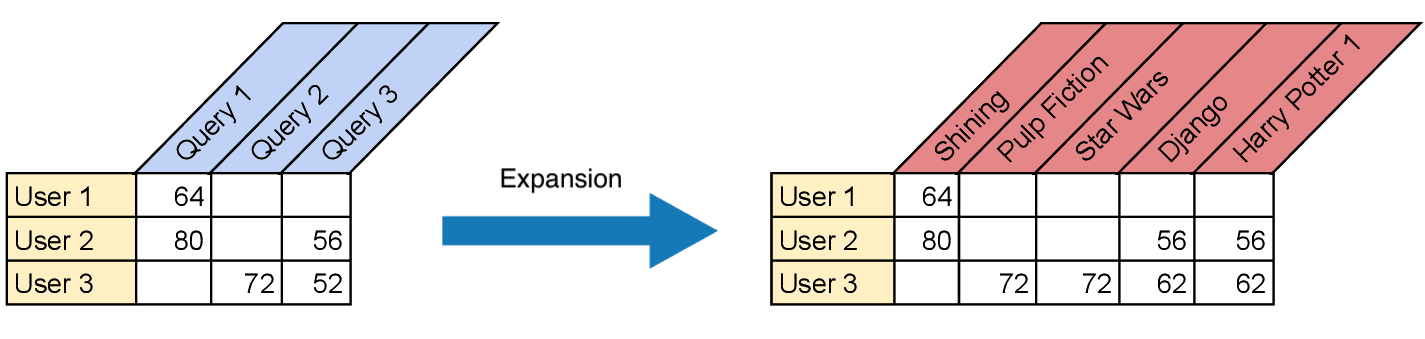
\includegraphics[width=8.5cm]{Data Mining/images/expansion.png}
\caption{Expansion Users-Queries Utility Matrix into Partial Users-Items Utility Matrix}
\label{fig:expansion}
\end{figure}

\subsubsection{Item-Item collaborative filtering execution on the users-
items utility matrix}
\label{sec:expanded-cf}
In this step, the main objective regards filling the \textit{users-item\_utility\_matrix} previously computed in order to obtain a complete matrix in which each row $u$ represents a user, each column $i$ represents an item and each cell ($u$,$i$) represents a rating prediction of the user $u$ for the relational item $i$.

To fill the \textit{users-item\_utility\_matrix} it was used the same \textbf{Item-Item Collaborative Filtering} approach described in the subchapter \ref{sec:compact-item-item-cf-solution}, but, instead of using the Utility Matrix $U$ as input, were used the \textit{users-item\_utility\_matrix} itself. In Figure \ref{fig:item-ritem-cf} it is shown an example of the result obtained by doing so.

\begin{figure}[h!]
\centering
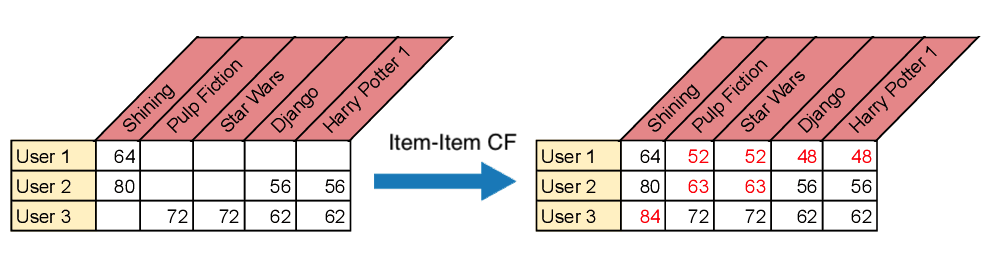
\includegraphics[width=8.5cm]{Data Mining/images/item-ritem-cf.png}
\caption{Item-Item Collaborative Filtering applied on the Expanded Utility Matrix}
\label{fig:item-ritem-cf}
\end{figure}

\subsubsection{Compression users-items to users-queries utility matrix} \label{ch:4.2.3}
Once the \textit{users-item\_utility\_matrix} was filled, as previously described, it was used to compute the \textit{complete users-queries\_utility\_matrix}, the requested output of the problem statement. This \textbf{compression} phase was performed by taking each user-query combination, by \textbf{identifying the items} that will be part of the result set of the query previously considered (referring to the \textit{preprocessed\_queries} matrix computed in Algorithm \ref{alg:preprocessing_queries}) and by computing the \textbf{mean} of the ratings of those items for the specific user in consideration. Those ratings are actually read from the complete \textit{users-item\_utility\_matrix} computed in the subsection \ref{sec:expanded-cf}. In order to improve both the performance in time of this compression, both its correctness, if a user-query combination was already known from the Utility Matrix $U$ given as input of the problem, those satisfaction values were also reported in the complete \textit{users-queries\_utility\_matrix} without compute any other operation. In pseudo-code, the complete \textit{users-queries\_utility\_matrix} is computed as described in Algorithm \ref{alg:reduction user-item}.

\begin{algorithm}
\caption{Complete users-queries\_utility\_matrix computation}\label{alg:reduction user-item}
\KwData{users,items,queries,utility\_matrix,users-item\_utility\_matrix,preprocessed\_queries}
\KwResult{users-queries\_utility\_matrix}

users-queries\_utility\_matrix[][] \\
\For{user \textbf{in} users}{
    \For{query \textbf{in} queries}{  
        item\_counter=0 \\
        partial\_rating=0 \\
        \uIf{utility\_matrix[user][query]==""}{
            \For{item \textbf{in} items}{    
               \uIf{preprocessed\_queries[query][item]==True}{
                    partial\_rating+= users-item\_utility\_matrix[user][item]
                    item\_counter+=1 \\
                }
            }
            users-queries\_utility\_matrix[user][query]= partial\_rating  /item\_counter \\
        }\Else{
            users-queries\_utility\_matrix[user][query]= utility\_matrix[user][query]
        }
    }
      
}
\end{algorithm}

The \textit{users-queries\_utility\_matrix} is actually complete because every user has expressed, in the \textit{users-item\_utility\_matrix}, a rating toward any item. This has as consequence that every item that compose the result of any query will be rated, and so computing the mean of those items ends up in being a trivial operation. This \textit{users-queries\_utility\_matrix}, for how it was intended during the expansion part described in the subchapter \ref{sub:expansion}, is \textbf{more reliable} in predicting the preferences regarding the queries that involves a relatively \textbf{small amount of items} in comparison to the cardinality of the entire Relational Table given as input. In Figure \ref{fig:compression} it is shown an example of the result of the compression described.

\begin{figure}[h!]
\centering
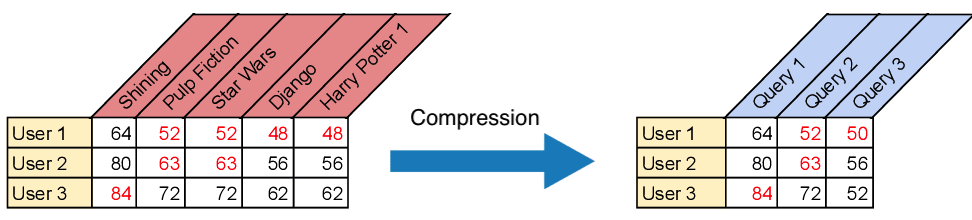
\includegraphics[width=8.5cm]{Data Mining/images/compression.png}
\caption{Compression Complete Users-Items Utility Matrix into Complete Users-Queries Utility Matrix}
\label{fig:compression}
\end{figure}

\subsection{Hybridization}
\label{cap:hybridization}
The final solution exploits the two previously computed \textit{Complete Utility Matrices} by both the \textbf{Compact Item-Item} Collaborative Filtering and \textbf{Expanded Item-Item} Collaborative Filtering components with a linear combination of their ratings driven by \textbf{query result cardinality}.
More precisely, based on the number of tuples belonging to the result set of a specific query, a different weight is assigned to the ratings of the same cell (user, query) of the two \textit{Complete Utility Matrices} to obtain a new rating.
Therefore, this rating takes into account both the rating calculated with Compact and Expanded Item-Item CF components, but with a \textbf{different weight} based on how many results are returned by the corresponding query.

In order to count the values of the result set of each query, an intermediate utility file, which is already used for the Expanded Item-Item Collaborative Filtering component and described in Section \ref{sub:expansion}, is exploited.
Leveraging the fact that each row, representing a query, acts like a BitSet of the items present in the correspondent query result set (its value is \textit{True} if the item is present), the cardinality is easily computed.
This cardinality, compared with \textbf{thresholds}, is used as discriminator for the choice of the \textbf{weights}, as illustrated in Algorithm \ref{alg:hybrid}.

There are \textbf{several ways} to assign weights and thresholds. The most accurate method of assigning them may change due to inherent hidden concepts of the particular dataset, the shape and characteristics of the dataset itself (e.g. mean, minimum, maximum of the result set cardinality). 
Each of these options needs to be carefully considered on a case-by-case basis in order to select the best way to proceed for the context being examined and finally to be able to fine-tune the parameters.

\textbf{One path} that could be chosen, that is the current one used for the evaluation experiments, consists in giving more weight to the rating provided by the \textit{Utility Matrix} of the Compact method if the query result set’s \textbf{cardinality is high}; instead, if that \textbf{cardinality is low}, a greater weight is given to the rating provided by the \textit{Utility Matrix} of the expanded method.  
Thresholds must be chosen having a clue of the mean, minimum and maximum value of the queries' result sets of the dataset analyzed, in order to achieve a \textbf{coherent splitting} of the 3 possible linear combination. For instance, if the higher threshold is set to a value higher than the widest query result set cardinality, then the first linear combination would be never used in the computation. 
For the current dataset the mean value of the result set cardinality is 221, the minimum value is 0 and the maximum value is 4696. 
Therefore the 2 threshold chosen, that are consistent with the characteristics described above, are 200 (lower bound) and 1000 (upper bound).
The three weights were chosen in such a way that the combinations did not lean too heavily toward a single approach but were \textbf{symmetrically balanced} with one another. Therefore the weights chosen and currently used are: 0.75, 0.50, 0.25 and they are used in a symmetric way as show in Algorithm \ref{alg:hybrid}.



\begin{algorithm}
\caption{Linear combination of Expanded Item-Item Collaborative Filtering and Compact Item-Item Collaborative Filtering}
\label{alg:hybrid}
\KwData{preprocessed\_queries, THRESHOLD\_1, THRESHOLD\_2, WEIGHT\_1, WEIGHT\_2, WEIGHT\_3}
\KwResult{hybrid\_utility\_matrix}
\For{query \textbf{in} queries}{

results\_in\_query[query] = \\preprocessed\_queries[query].value\_counts())

}


\For{query \textbf{in} queries}{

    \uIf{results\_in\_query[query] >= THRESHOLD\_2}{
        compact\_CF\_weight = WEIGHT\_1 
        
        expanded\_CF\_weight = 1 - WEIGHT\_1 
    }
    \uElseIf{results\_in\_query[query] < THRESHOLD\_2 \\
    \&\& results\_in\_query[query] > THRESHOLD\_1}{
        compact\_CF\_weight = WEIGHT\_2 
        
        expanded\_CF\_weight = 1 - WEIGHT\_2 
    }
    \Else{
        compact\_CF\_weight = WEIGHT\_3
        
        expanded\_CF\_weight = 1 - WEIGHT\_3 
    }

    \For{user \textbf{in} users}{
    hybrid\_utility\_matrix[user][query] = compact\_CF\_weight * compact\_CF\_utility\_matrix[user][query] + \
    expanded\_CF\_weight * expanded\_CF\_utility\_matrix[user][query]
    }
}
\end{algorithm}

The \textit{hybrid\_utility\_matrix} that can be computed with the above mentioned algorithm, is the \textit{Complete Utility Matrix} requested as \textbf{output} in the problem statement.


\subsection{Leverage the final solution to solve PART A}

The first goal met by the proposed solution is to generate a \textit{Complete Utility Matrix}. Directly related to this first objective, one can use the tool to obtain the \textit{Top-K} queries that may be of interest to the user $u$. The parameters $k$ and $u$ are therefore the input parameters of this component of the solution, referred to as \textbf{PART\_A}.

In order to perform the above described task, the user row is scanned in the \textit{Complete Utility Matrix} proposed and the \textit{Top-K} queries are given as output. The viewer can choose whether to receive only new ratings or ratings that were also previously present in the initial (sparse) \textit{Utility Matrix} $U$.


\subsection{Leverage the final solution to solve PART B}
The \textbf{PART\_B} of the project asks to develop a more general solution that is able, given some \textbf{unseen queries}, to compute a preference score about them for each user belonging to the User Set $US$ in input. Another way to interpret the task is to fill a new \textit{Utility Matrix}, so such was requested in \textbf{PART\_A}, composed by the matrix $U$ to which are appended some queries that are not rated by any users, and so that will have their corresponding column composed only by \textit{NULL} values. The solution proposed, that will be described in details in the following subchapters, use the results achieved by the PART\_A in order to compute a new \textit{users-RelationalItem\_utility\_matrix}, whose ratings are combined in order to give a prediction regarding new unseen queries.

\subsubsection{Expansion user-item}
The first operation done in order to achieve the \textbf{PART\_B} goal, as previously mentioned, is the computation of a new \textit{users-RelationalItem\_utility\_matrix}, starting from the output computed by the procedure developed in the PART\_A. This expansion follows the same underlying idea described in the subchapter \ref{sec:expansion}, even if some differences occurs due to the fact that:

\begin{itemize}
    \item The matrix used as starting point for the expansion is \textbf{complete} and so all the users will have a preference score, in the computed \textit{users-RelationalItem\_utility\_matrix}, about the same items. The score regarding the relational tuples, indeed, is retrieved by shifting the rating of a query to their results and there are not users, in the matrix obtained in PART\_A, that have rated some queries that others won't.
    \item In the expanded \textit{users-RelationalItem\_utility\_matrix} there could exists, by the way, some items that still not have a rating: it is indeed possible that some queries present in the Utility Matrix $U$, and so also in the \textit{Complete Utility Matrix} obtained from PART\_A, won't have returned some items belonging to the relational table taken into account. It is also not possible to use any collaborative filtering approach because all the users will have the cells belonging to those items \textbf{empty}. In order to fill those users-items combinations in a coherent way, it is assigned, in those cases, a score equal to the mean of the other scores expressed by the user considered for the rated relational items.
\end{itemize}
The algorithm used in order to achieve this aim is very similar to Algorithm \ref{alg:expansion-user-queries} and differs from it only for managing the previous observations, by introducing a new behavior in the case the variable \textit{denominator} will be equal to 0. The pseudocode following those steps is illustrated in Algorithm \ref{alg:partb-ch4.5.1}, where the parameter \textit{utility\_matrix} requested as input represent the \textit{Complete Utility Matrix} computed in \ref{cap:hybridization}.

\begin{algorithm}
\caption{PART\_B users-RelationalItem\_utility\_matrix computation}\label{alg:partb-ch4.5.1}
\KwData{preprocessed\_queries, users, items, queries,utility\_matrix}
\KwResult{users-RelationalItem\_utility\_matrix}
n\_results[] \\
users-RelationalItem\_utility\_matrix[][] \\
\For{query \textbf{in} queries}{
    n\_results[query] = preprocessed\_queries[query].count() \\
}
\For{user \textbf{in} users}{
     
    \For{item \textbf{in} items}{
        \For{query \textbf{in} queries}{
            \If{utility\_matrix[user][query]}{
                current\_weight=n\_results[query]
                total\_weight+=current\_weight \\
            }  
        }
        \For{query \textbf{in} queries}{
            \If{utility\_matrix[user][query]}{
                partial\_score+=utility\_matrix[user][query] * total\_weight / n\_results[query]
                denominator+=total\_weight / n\_results[query] \\
            }  
        }
        \uIf{denominator!=0}{
            users-RelationalItem\_utility\_matrix[user][item]=partial\_score / denominator \\
        } \Else{
            users-RelationalItem\_utility\_matrix[user][item]= "PLACEHOLDER"
        }
      
    }
    rating\_mean=0 \\
    item\_counter=0

    \For{item \textbf{in} items}{ \\
        \If{users-RelationalItem\_utility\_matrix[user][item]!= "PLACEHOLDER"}{\\
            rating\_mean+= users-RelationalItem\_utility\_matrix[user][item] \\
            item\_counter+=1 \\
        } \\
    }\\
    rating\_mean=rating\_mean/item\_counter\\
    \For{item \textbf{in} items}{ \\
        \If{users-RelationalItem\_utility\_matrix[user][item]== "PLACEHOLDER"}{ \\
            users-RelationalItem\_utility\_matrix[user] [item]=rating\_mean
        } \\
    } \\
} \\
\end{algorithm}

\subsubsection{Score computation}
Once that the \textit{users-RelationalItem\_utility \_matrix} is computed, it is possible, given some new unseen queries, to compute their preference scores by:
\begin{itemize}
    \item \textbf{checking} whose items of the relational table represent a result for each given query. This procedure is accomplished by executing Algorithm \ref{alg:preprocessing_queries} to which the list \textit{queries}, requested as input, represent the new queries introduced.
    \item \textbf{computing}, for each user $u$, the mean of the scores that he assigned to the relational tuples composing the results of each new query $q$ given. This result will be the one to be assigned to the cell ($u$,$q$) of the matrix in output.
\end{itemize}
The relative \textit{users-queries\_utility\_matrix}, computed by executing Algorithm \ref{alg:reduction user-item} with \textit{users-RelationalItem\_utility \_matrix} as input, will be the output requested by \textbf{PART\_B}. In order to replicate the entire procedure we will refer to Algorithm \ref{alg:preprocessing_queries} with the new queries as input, for obtaining the BitSet \textit{new\_preprocessed\_queries}, and to Algorithm \ref{alg:partb_ch4.5.2}, for getting the \textit{Complete Utility Matrix} requested by PART\_B.

\begin{algorithm}
\caption{PART\_B users-queries\_utility\_matrix computation}\label{alg:partb_ch4.5.2}
\KwData{new\_preprocessed\_queries, users, items, queries,utility\_matrix}
\KwResult{users-queries\_utility\_matrix}
users-queries\_utility\_matrix[][] \\

\For{user \textbf{in} users}{
    \For{query \textbf{in} queries}{
        partial\_query\_score=0 \\
        results\_counter=0 \\
        \For{item \textbf{in} items}{
            \If{new\_preprocessed\_queries[query][item]==True}{
                partial\_query\_score+=users-RelationalItem\_utility\_matrix[user][item]\\
                results\_counter+=1 \\
            }\\  
        }
        \uIf{results\_counter!=0}{
            users-queries\_utility\_matrix[user][queries]= partial\_query\_score / results\_counter\\
        }\Else{
            users-queries\_utility\_matrix[user][queries]=0\\
        }\\
      \\
    } \\
}
\end{algorithm}

The \textit{users-queries\_utility\_matrix}, obtained by the execution of the previous algorithms, satisfies the PART\_B of the project. Indeed, it has at each row $u$ each user presents in the user set $US$ taken as input, at each column $q$ each new queries proposed and, finally, in each cell ($u$,$q$) a prediction about the preference score of the user $u$ for the new \textbf{unseen} query $q$ based on the \textbf{users history}.





\subsection{Further improvements}

\textbf{Clustering} and dimensionality reduction techniques could improve temporal performance in the \textit{Utility Matrix}'s pre-computing phase of the current solution.
However, as stated in the introduction section of Chapter \ref{sec:solution}, the proposed solution was assumed to be in an offline context. As a result, on-demand requests for PART\_A and PART\_B tasks use pre-computed data that is saved on disk in the form of ".csv" files.

\subsection{Discarded approaches}

\subsubsection{User-User Collaborative Filtering}
The User-User Collaborative Filtering method yielded \textbf{lower performance} metrics for both the compact and expanded versions, as it can be seen is Section \ref{sec:compact-user-user-metrics}. This confirmed what was discovered in the analysis of related works in Chapter \ref{sec:related_work}: Item-Item Collaborative Filtering typically outperforms User-User Collaborative Filtering.

\subsubsection{Content-based method}

A \textbf{content-based} method was also implemented.
The initial strategy was to elect it as a method to be included in the final hybrid solution, as a weight portion, but \textbf{failed} some preliminary performance tests.

Although a fairly large number of options and alternatives were tested, good performance metrics were not obtained.

Best performances were achieved with the use of "dynamic profiles" that change based on what \textit{user-query} comparison is to be done.
Each user profile is composed of its \textit{TOP\_Q} values for each possible attribute plus the values present in the query attributes if not already present in the user profile. 





\newpage
\section{Experimental evaluation}
%\label{sec:context}

\subsection{Dataset composition}
The dataset taken into account during the experimental evaluation is composed both by \textbf{real} and \textbf{synthetic} data organized in ".csv" files. In particular the \textbf{Relational Table} $RT$ is composed by real data that, in the scenario considered, represents 7669 existing movies. The movies taken into account were retrieved from kaggle.com, a popular collection of public datasets used for data science works. The dataset was moreover cleaned and projected in the tuple $\langle name, genre, runtime, year, country, score \rangle$ \\in order to make it compatible with the other synthetic data used.
The \textbf{User Set} $US$, the \textbf{Query Set} $QS$ and the \textbf{Utility Matrix} $U$ are instead synthetic and were generated by the team. In particular:
\begin{itemize}
    \item The \textbf{User Set} is composed by a list of 2500 users' ids generated through the use of the $uuid$ python's module. Each user has an \textbf{unspoken preference} regarding each attribute belonging to the items' tuple in order to generate the utility matrix in a \textbf{coherent} way. 
    \item The \textbf{Query Set} is composed by 100 queries. Each query is represented by at least a key-value constraints, where each one of them corresponds to existing attribute and value present in at least a tuple of the Relational Table $RT$. 
    \item The \textbf{Utility Matrix} is composed by a matrix having $u$ rows, with $u$ corresponding to the number of users, and $q$ columns, with $q$ corresponding to the number of queries. \textbf{One third} of the user-query combinations of the matrix is filled with a rating computed by taking into account the unspoken user preferences on the results produced by the execution of the queries on the relational table.
\end{itemize}
The \textit{Complete Utility Matrix}, composed by the Utility Matrix $U$ without any hidden value, was also stored in order to use it only during the \textbf{performance evaluation} of the proposed solution and of the ones produced by the baselines considered.

\subsection{Dataset generation} \label{ch:5.2}
The synthetic data of the dataset considered were generated in order to accomplish the attributes and values of the real relational table. Another choice taken, in order to work on a dataset having as \textbf{few assumptions} as possible and so whose solution would work in the same way also with other ones, was to do \textbf{not} establish any correlation through different distances between the values belonging to discrete fields. For instance, in the current scenario, the Thriller genre could have been considered a closer concept to the Horror genre than the Musical genre.

\subsubsection{Fields recognition}
In order to generate the data in this way, first of all it was necessary to analyze the kind of attributes belonging to the real relational table and to divide them in:
\begin{itemize}
    \item \textbf{Discrete Attribute} (as the genre and the country)
    \item \textbf{Continuous Attributes} (as the runtime, the publication year and the score)
    \item \textbf{Not-relevant attributes} (as the "name")
\end{itemize}
In order to do that, the distinction was computed by considering at first the attributes where each of their value could be parsed in a numeric format. Those fields were considered as \textbf{continuous}. The non-continuous fields, in addition, were divided in \textbf{not-relevant} attributes, in the case they were unique in at least the 75\% of the times, and \textbf{discrete}, otherwise. During the generation of the dataset it is also given the possibility of specifying manually which continuous fields will influence the user ratings in the same way for everyone, for example in the current relational table the field "score" (like a IMDB score) will influence everyone \textbf{in the same way} by increasing or decreasing the rating given to an item independently by the users' preferences.

\subsubsection{User profiles}
Once the fields were divided in this way, they were leveraged in order to build the users' profiles. Each user's profile is characterized by:
\begin{itemize}
    \item a \textbf{user\_id}, which represents the only known field about the user used by the actual solution algorithm.
    \item an \textbf{average\_score\_translation} field, a random value between -10 and 10 that will indicate if a user is \textbf{severe or not} in his rating.
    \item \textbf{10 fields for every discrete field} of the relational table, in order to indicate which are the values for those fields that a user will \textbf{appreciate} the most (the first 4 ones) or the least (the last 6 ones). The values not present in the user profile will be simply rated as unpleasant, with a contribution of 60 out of 100 each.
    \item \textbf{a field for every continuous attribute} regarding the items (except for the score one), in order to express the users' unspoken preferences toward a certain continuous item field. Those preferences contains a value picked from a \textbf{Gaussian distribution} having as mean the mean value regarding a certain continuous attribute and with a standard deviation such that over the 98,5\% of the values will be in the range of values found in the relational table for each attribute. It was chosen to use a Gaussian distribution in order to generate those preferences by also managing the existence of very high or very low values appearing in the big minority of the items considered. If it was chosen to pick some random equiprobable values for computing the users' preferences between the real range of values, a big amount of those picks will be strongly similar to only few (usually one) items of the relational table.
\end{itemize}
Those users profiles built were used both in the creation of the Utility Matrix $U$ belonging to the input of the problem, both during the evaluation performed for the PART\_B of the solution proposed.

\subsubsection{Query definition}
It was then built the definition of the attribute-value constraints belonging to 100 queries that will compose the columns of the utility matrix proposed. In order to reduce the number of queries that won't return any result if executed on the Relational Table $RT$, after having picked a attribute-value constraint referring to a considered field present in the relational table, the other ones were added with 25\% of probability each. The combination of those constraints will represent our query definition.

\subsubsection{Query result computation}
As a pre-computation used during the creation of the Utility Matrix, each query was computed on the entire relational table and its results were saved in a file called \textit{*query\_id*.csv}. This operation was simply done by iterating over all the attribute-value pairs defined for each query and by writing to file the items that were satisfying all of it.

\subsubsection{Utility matrix computation}
With all those computations performed, it is actually possible to compute both the \textit{Real Utility Matrix}, a complete matrix containing the ratings of all the users for all the queries, both the \textit{Utility Matrix} $U$, that represents an \textbf{input} of our problem statement.
In order to compute them, an iteration through all the users and all the query results achieved was performed and it was assigned, using the unspoken preferences of the users, a rating for each query. The rating of a query by a user corresponded to the \textbf{mean} of all the ratings that the user gave to its \textbf{results}. The rating given to a single item by a user is obtained by the sum of:
\begin{itemize}
    \item the ratings given to each \textbf{discrete attribute} of the item. Those ratings depend by the position of which the effective discrete value of an item appears in the user profile.
    \item the ratings given to each \textbf{continuous attribute} of the item. Those ratings depend on the distance between the value characterizing an item and the one presents in the user preferences. It was chosen to use an arithmetic distance normalized considering the values' spectrum of each attribute taken into account in order to obtain a preference score between 0 and 100. This distance obtained it was furthermore subtracted to 100 in order to have an higher value when the user profile and the item's one were similar.
    \item a value indicating how the item in account was \textbf{generally} appreciated. This value is represented, in our case, by the $score$ field that can also influence negatively the rating assigned to an item. This field was normalized in order to give to it the possibility to add a value between -7,5 and 7,5 to the final score assigned to the item.
\end{itemize}
After having summed up the previous values, the final result was normalized in order to obtain a value between \textbf{0 and 100} by dividing it by the number of the considered items' fields taken into account (excluded the \textit{score} one that was managed in a different way). The case in which a rating was still over 100 or under 0 were shifted respectively to 100 and to 0.

The mean of the ratings, belonging to items composing the results of the same query, will \textbf{compose the rating} assigned by a user to the query taken into account. In order to provide more variety between the queries ratings assigned by different users, it was furthermore added to it:
\begin{itemize}
    \item the \textit{average\_score\_translation} belonging to each user profile, a value between -10 and 10 used to indicate if a user is \textbf{severe or not} in his reviews.
    \item a \textbf{random noise} between -5 and 5, in order to get less predictable results.
\end{itemize}
Also this obtained rating was shifted in order to get a value between 0 and 100. The pseudocode related to this rating-computation procedure is illustrated with Algorithm \ref{alg:users-queries score computation}.

\begin{algorithm}
\caption{Utility Matrix and Complete Utility Matrix Computation}
\label{alg:users-queries score computation}
\KwData{users,query\_results (by reading each \textit{*query\_id*.csv}),queries,utility\_matrix,preprocessed\_queries, DISC\_FIELDS,CONT\_FIELDS,SCORE}
\KwResult{utility\_matrix,complete\_utility\_matrix}

complete\_utility\_matrix[][] \\
utility\_matrix[][] \\

\For{user \textbf{in} users}{ 
    \For{query \textbf{in} queries}{ 
        partial\_query\_rating=0 \\
        \For{item \textbf{in} query\_results[query]}{
            partial\_item\_rating=0 
            
            \For{field \textbf{in} item}{ 
                \If{field in DISC\_FIELDS}{ 
                    partial\_query\_rating+= compute\_discrete(user[field],item[field]) 
                }
                \uIf{field in CONT\_FIELDS \&\& field \textbf{not in} SCORE}{ 
                    partial\_query\_rating+= compute\_continuous(user[field],item[field]) 
                }\Else{ 
                    partial\_query\_rating+= compute\_score(item[field]) 
                }
            } 
        } 

        partial\_query\_rating+= partial\_item\_rating / (|DISCR\_FIELD|+| CONT\_FIELDS|-|SCORE|)

    partial\_query\_rating=partial\_query\_rating / query\_results[query].len() 
    
    partial\_query\_rating+=user["average\_score\_translation"] 
    
    final\_query\_rating=partial\_query\_rating+random(-5,5) 
    
    complete\_utility\_matrix[user][query] = final\_query\_rating
    
    \If{random(1,3)==1}{ 
        utility\_matrix[user][query] = final\_query\_rating 
    } 
    }
        
} 

%return partial\_utility\_matrix,real\_complete\_utility\_matrix

\end{algorithm}





The \textit{compute\_discrete(user[field],item[field])} function in \ref{alg:users-queries score computation} checks in which position, if it exists, a discrete value of the relational tuple appears in the user profile. In particular, if a value appears in the first 4 positions of the user profile regarding the attribute considered, the rating given is between 100 and 70, according to its exact position. If the value instead appears in the last 6 positions, the rating given is poor, between 50 and 0. If the rating regarding a value does not appear in the user profile, it has a \textbf{standard contribution} of 60.
\textit{compute\_continuous(user[field],item[field])} is a function that computes the rating contribution regarding a continuous field that characterize the relational table in this way:
$$100-\frac{(abs(float(item[field])-float(user[field]))}{((max(field)-min(field))/100))}$$
So, it computes an arithmetic distance between the user preference and the item value regarding the same continuous field and it normalizes it in order to obtain a value between 0 and 100. It is also computed the complementary of this distance in order to obtain a similarity value.

\textit{compute\_score(item[field])} normalize the \textit{item[field]} in a value between -7.5 and 7.5. 

Finally, because the scores (belonging to the "score" field) in our dataset were between 0 and 5, the relative computation was performed in the following way:
$$(float(item[field])-2.5)*3$$

In this way, it is possible to compute all the ratings belonging to each user-query combination that will be part of the real and complete utility matrix used during the evaluation process. By \textbf{randomly keeping only the 33\%} of those ratings it is possible to obtain, instead, the Utility Matrix $U$ used during the solution's idealization.

\subsection{Dataset independence}

The solution provided is \textbf{independent} from the default input dataset.
This priority in building a general solution was considered since the \textbf{dataset generation}, whose algorithm adapts itself based on the type of values present in the \textbf{relational table} proposed as starting point. With the same approach, were also developed all the strategies that were tried for both the PART\_A and the PART\_B of the problem statement such that, every input given with the requested ".csv" representation, will be accepted independently by its fields and its cardinality.


\subsection{Evaluation metrics}
\label{sec:evaluation-metrics}

The evaluation metrics taken into account were:
\begin{itemize}
  \item \textbf{Mean Absolute Error} (MAE)
  \item \textbf{Root Mean Squared Error} (RMSE)
  \item \textbf{Mean Absolute Percentage Error} (MAPE)
\end{itemize}

\subsubsection{MAE}
In statistics, Mean Absolute Error (MAE) is a measure of errors between paired observations expressing the same phenomenon. \cite{MAE} In this particular case, Y versus X is the comparison of real value versus predicted. MAE is calculated as the sum of absolute errors divided by the sample size:

$$MAE = \frac{\sum ^{n}_{i=1} \left | y_{i} - x_{i} \right |}{n} = \frac{\sum ^{n}_{i=1} \left | e_{i}  \right |}{n}$$

In other words, its result show how close the predictions ($x_i$) are to the actual model ($y_i$) on average.
Low MAE values indicate that the model is correctly predicting. Larger MAE values indicate that the model is poor at prediction. \cite{metrics}

\subsubsection{RMSE}

The Root Mean Squared Error (RMSE) is the square root of the average of squared errors. The effect of each error on RMSE is proportional to the size of the squared error; thus RMSE is sensitive to \textbf{outliers}. \cite{RMSE}

$$RMSE = \sqrt{\frac{\sum_{t=1}^{N}(A_t - F_t)^{2}}{N}}$$

RMSE is used to determine whether there are any large errors or distances that could be caused if the model overestimated the prediction (that is, the model predicted values that were significantly higher than the actual values) or underestimated the predictions (that is, predicted values less than actual values). \cite{metrics}



\subsubsection{MAPE}

The Mean Absolute Percentage Error (MAPE) is another measure of prediction accuracy of a forecasting method in statistics. It usually expresses the accuracy as a ratio defined by the formula:

$$MAPE = \frac{100\%}{n} \sum_{t=1}^{n}\left | \frac{A_t - F_t}{A_t}  \right | $$

where $A_t$ is the actual value and $F_t$ is the forecast value. Their difference is divided by the actual value $A_t$. The absolute value of this ratio is summed for every forecasted point in time and divided by the number of points $n$.

According to some studies, a MAPE less than 5\% could be considered as an indication that the forecast is acceptably accurate. A MAPE greater than 10\% but less than 25\% could indicate low, but acceptable accuracy and MAPE greater than 25\% very low accuracy, so low that the forecast is not acceptable in terms of its accuracy. \cite{MAPE_VALUES}


These 3 metrics were used to \textbf{compare} the \textit{Real Complete Utility Matrix} (available right after the dataset generation) with the \textit{Complete Utility Matrix} computed by the final solution (Algorithm \ref{alg:hybrid}), and by the others approaches developed.

It should be noted that all of the aforementioned evaluation metrics are only ever used to compare two \textbf{full matrices}, one calculated by a developed component and the other created during the dataset generation phase.

In order to evaluate the tasks of PART\_A and PART\_B of the project, i.e., retrieve the \textit{TOP\_K} queries that may be of interest to the user $u$, \textbf{Jaccard similarity coefficient} were used.
This index is exploited to compare the \textbf{sets} of \textit{TOP\_K} queries computed from \textit{Real Complete Utility Matrix} and one computed with the developed algorithms.

\subsection{Experimental results accomplished by single components}

As said in the introduction of Chapter \ref{sec:solution}, the entire development process were driven not exclusively by reasoning deemed logical but also by empirical results. In this section, the \textbf{key experimental results} are reported.
Since the final solution relies on two separate components, it is helpful to examine their outcomes first.

\subsubsection{Compact Item-Item CF metrics values}

In order to determine the values of the three evaluation metrics mentioned in the previous section, the first experiments were carried out on the Compact Item-Item CF, the first component of the final solution.
Tables \ref{tab:compact Item-Item CF, nqueries fixed} and \ref{tab:compact Item-Item CF, nusers fixed} contain the results, and figures \ref{fig:Compact Item-Item CF, varying users} and \ref{fig:Compact Item-Item CF, varying queries} contain the relative plotted charts.
Regarding Figure \ref{fig:Compact Item-Item CF, varying users}, it is evident that all metrics considered in the chart reach a \textbf{plateau} after considering 200 users, even though the values are still slowly declining.
Figure \ref{fig:Compact Item-Item CF, varying queries} shows a slow decline in the metrics values rather than an initial steep section for the lower number of queries as there is for few users.

The data indicates that in order to reach a performance plateau, it is critical to cross a relatively consistent threshold of users, at least for this dataset. This behavior did not occur in the query variations considered.

\begin{table}[h!]
    \centering
    \begin{tabular}{ |p{2cm}||p{1.5cm}|p{1.5cm}|p{1.5cm}|  }
         \hline
         \multicolumn{4}{|c|}{Compact Item-Item CF, n\_queries (100) fixed } \\
         \hline
         \textbf{N\_USERS}& \textbf{MAE} &\textbf{RMSE} &\textbf{MAPE}\\
         \hline
         10 & 4.048 &  7.6871 & 8.7731\\
         20 & 3.7915 & 6.8982 & 8.2058\\
         50 & 3.6162 & 6.7762 & 8.3140\\
         100 & 3.3873 & 6.2586 & 7.5723\\
         200 & 3.3025 & 6.0730 & 7.2555\\
         300 & 3.2853 & 6.0379 & 7.2441\\
         400 & 3.2496 & 5.9567 & 7.1688\\
         500 & 3.2677 & 5.9896 & 7.2085\\
         1000 & 3.2384 & 5.9402 & 7.0622\\
         1500 & 3.2211 & 5.9151 & 7.0052\\ 
         2000 & 3.1691 & 5.8260 & 6.8783\\
         \textbf{2500} & \textbf{3.1420} & \textbf{5.7890} & \textbf{6.8218}\\
         
     
         \hline
    \end{tabular}
    \caption{Compact Item-Item CF, n\_queries fixed}
    \label{tab:compact Item-Item CF, nqueries fixed}
\end{table}


\begin{table}[h!]
    \centering
    \begin{tabular}{ |p{2cm}||p{1.5cm}|p{1.5cm}|p{1.5cm}|  }
         \hline
         \multicolumn{4}{|c|}{Compact Item-Item CF, n\_users (2500) fixed } \\
         \hline
         \textbf{N\_QUERIES}& \textbf{MAE} &\textbf{RMSE} &\textbf{MAPE}\\
         \hline
         10 & 3.2684 & 6.0499 & 7.5426\\
         20 & 3.1939 & 5.9215 & 7.3000\\
         30 & 3.1099 & 5.7911 & 7.0829\\
         40 & 3.0310 & 5.7740 & 7.2400\\
         50 & 3.2652 & 6.0235 & 7.2698\\
         60 & 3.3483 & 6.0666 & 7.1452\\
         70 & 3.1616 & 5.8735 & 7.0560\\
         80 & 3.2359 & 5.9161 & 6.9690\\
         90 & 3.2323 & 5.8874 & 6.8850\\
         \textbf{100}& \textbf{3.1420} & \textbf{5.7890} & \textbf{6.8218}\\
         
         \hline
    \end{tabular}
    \caption{Compact Item-Item CF, n\_users fixed}
    \label{tab:compact Item-Item CF, nusers fixed}
\end{table}

\begin{figure}[h!]
\centering
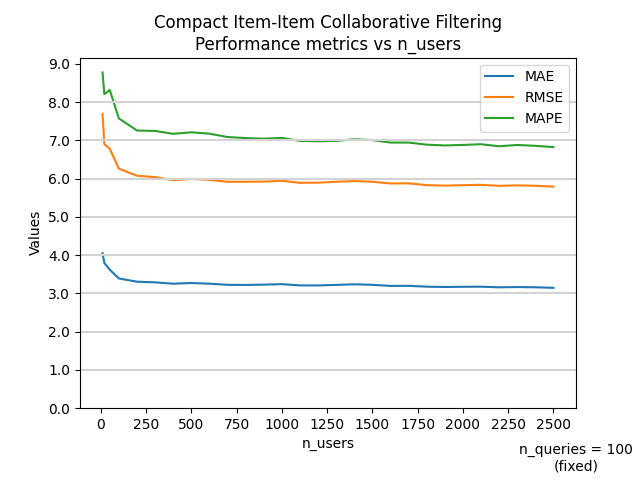
\includegraphics[width=9cm]{Data Mining/images/compact_item_item_users.png}
\caption{Evaluation metrics of Compact Item-Item CF, varying number of users}
\label{fig:Compact Item-Item CF, varying users}
\end{figure}

\begin{figure}[h!]
\centering
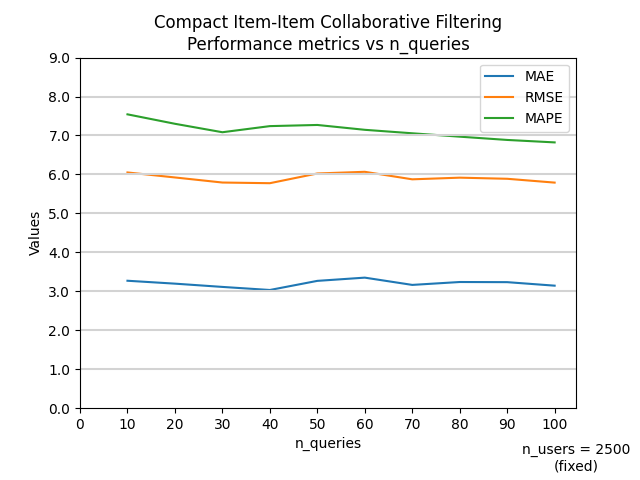
\includegraphics[width=9cm]{Data Mining/images/compact_item_item_queries.png}
\caption{Evaluation metrics of Compact Item-Item CF, varying number of queries}
\label{fig:Compact Item-Item CF, varying queries}
\end{figure}




\subsubsection{Compact User-User CF metrics values}
\label{sec:compact-user-user-metrics}

The experimental evaluation of Compact User-User Collaborative Filtering \textbf{confirmed what the theory says} about this topic, even in this specific setting: Item-Item CF often works better than User-User CF. As shown in Figures \ref{fig:Compact User-User CF, varying users} and \ref{fig:Compact User-User CF, varying queries}, all three metrics considered have significantly higher values than the values described in the previous section.

\begin{figure}[h!]
\centering
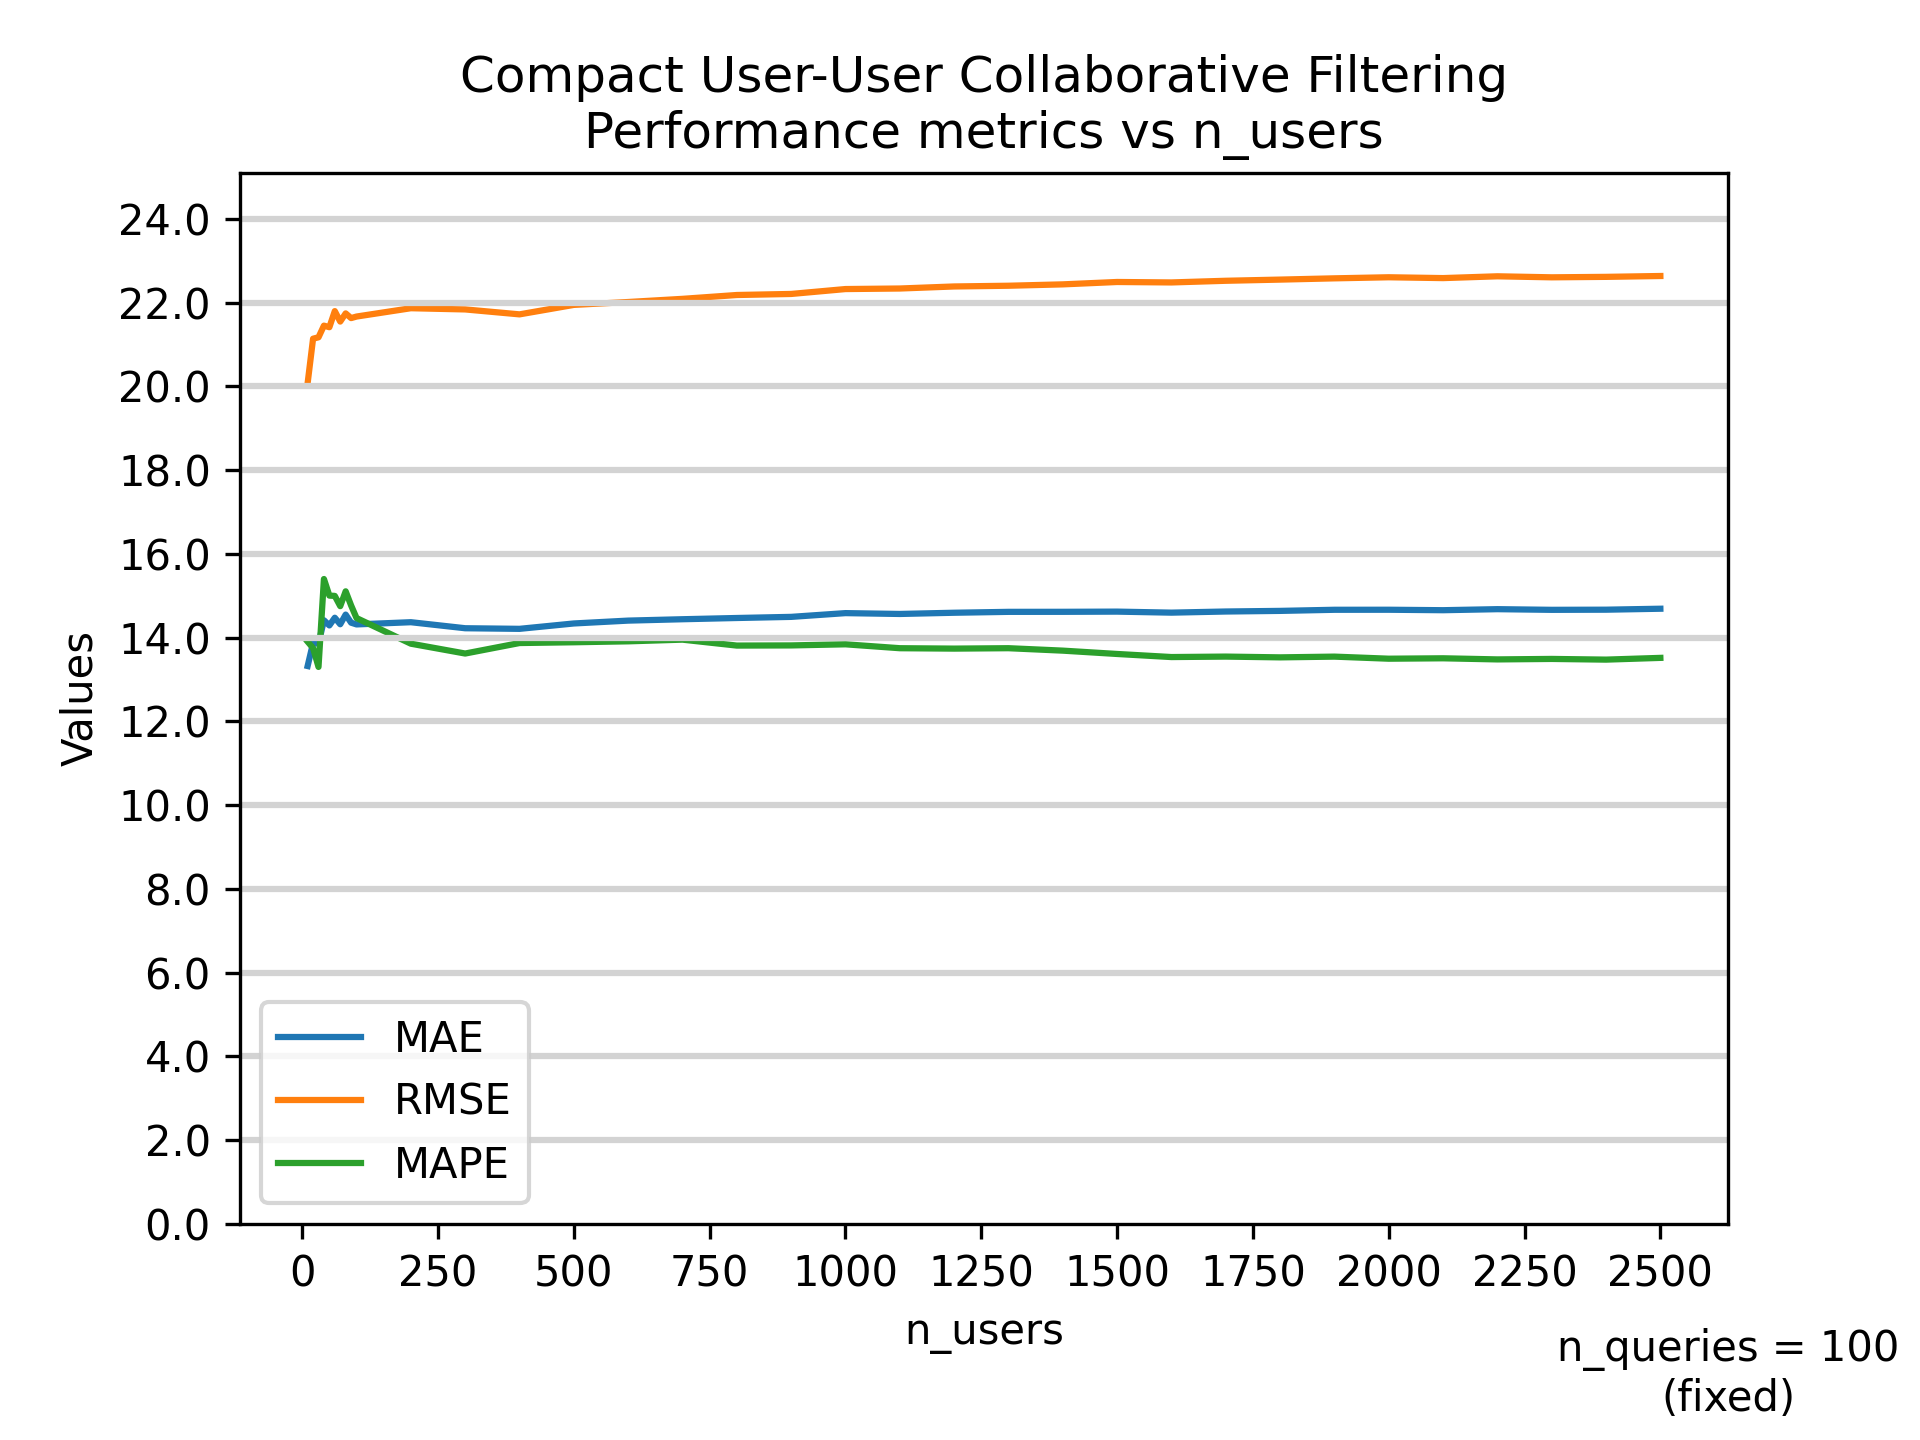
\includegraphics[width=9cm]{Data Mining/images/compact_user_user_users.png}
\caption{Evaluation metrics of Compact User-User CF, varying number of users}
\label{fig:Compact User-User CF, varying users}
\end{figure}

\begin{figure}[h!]
\centering
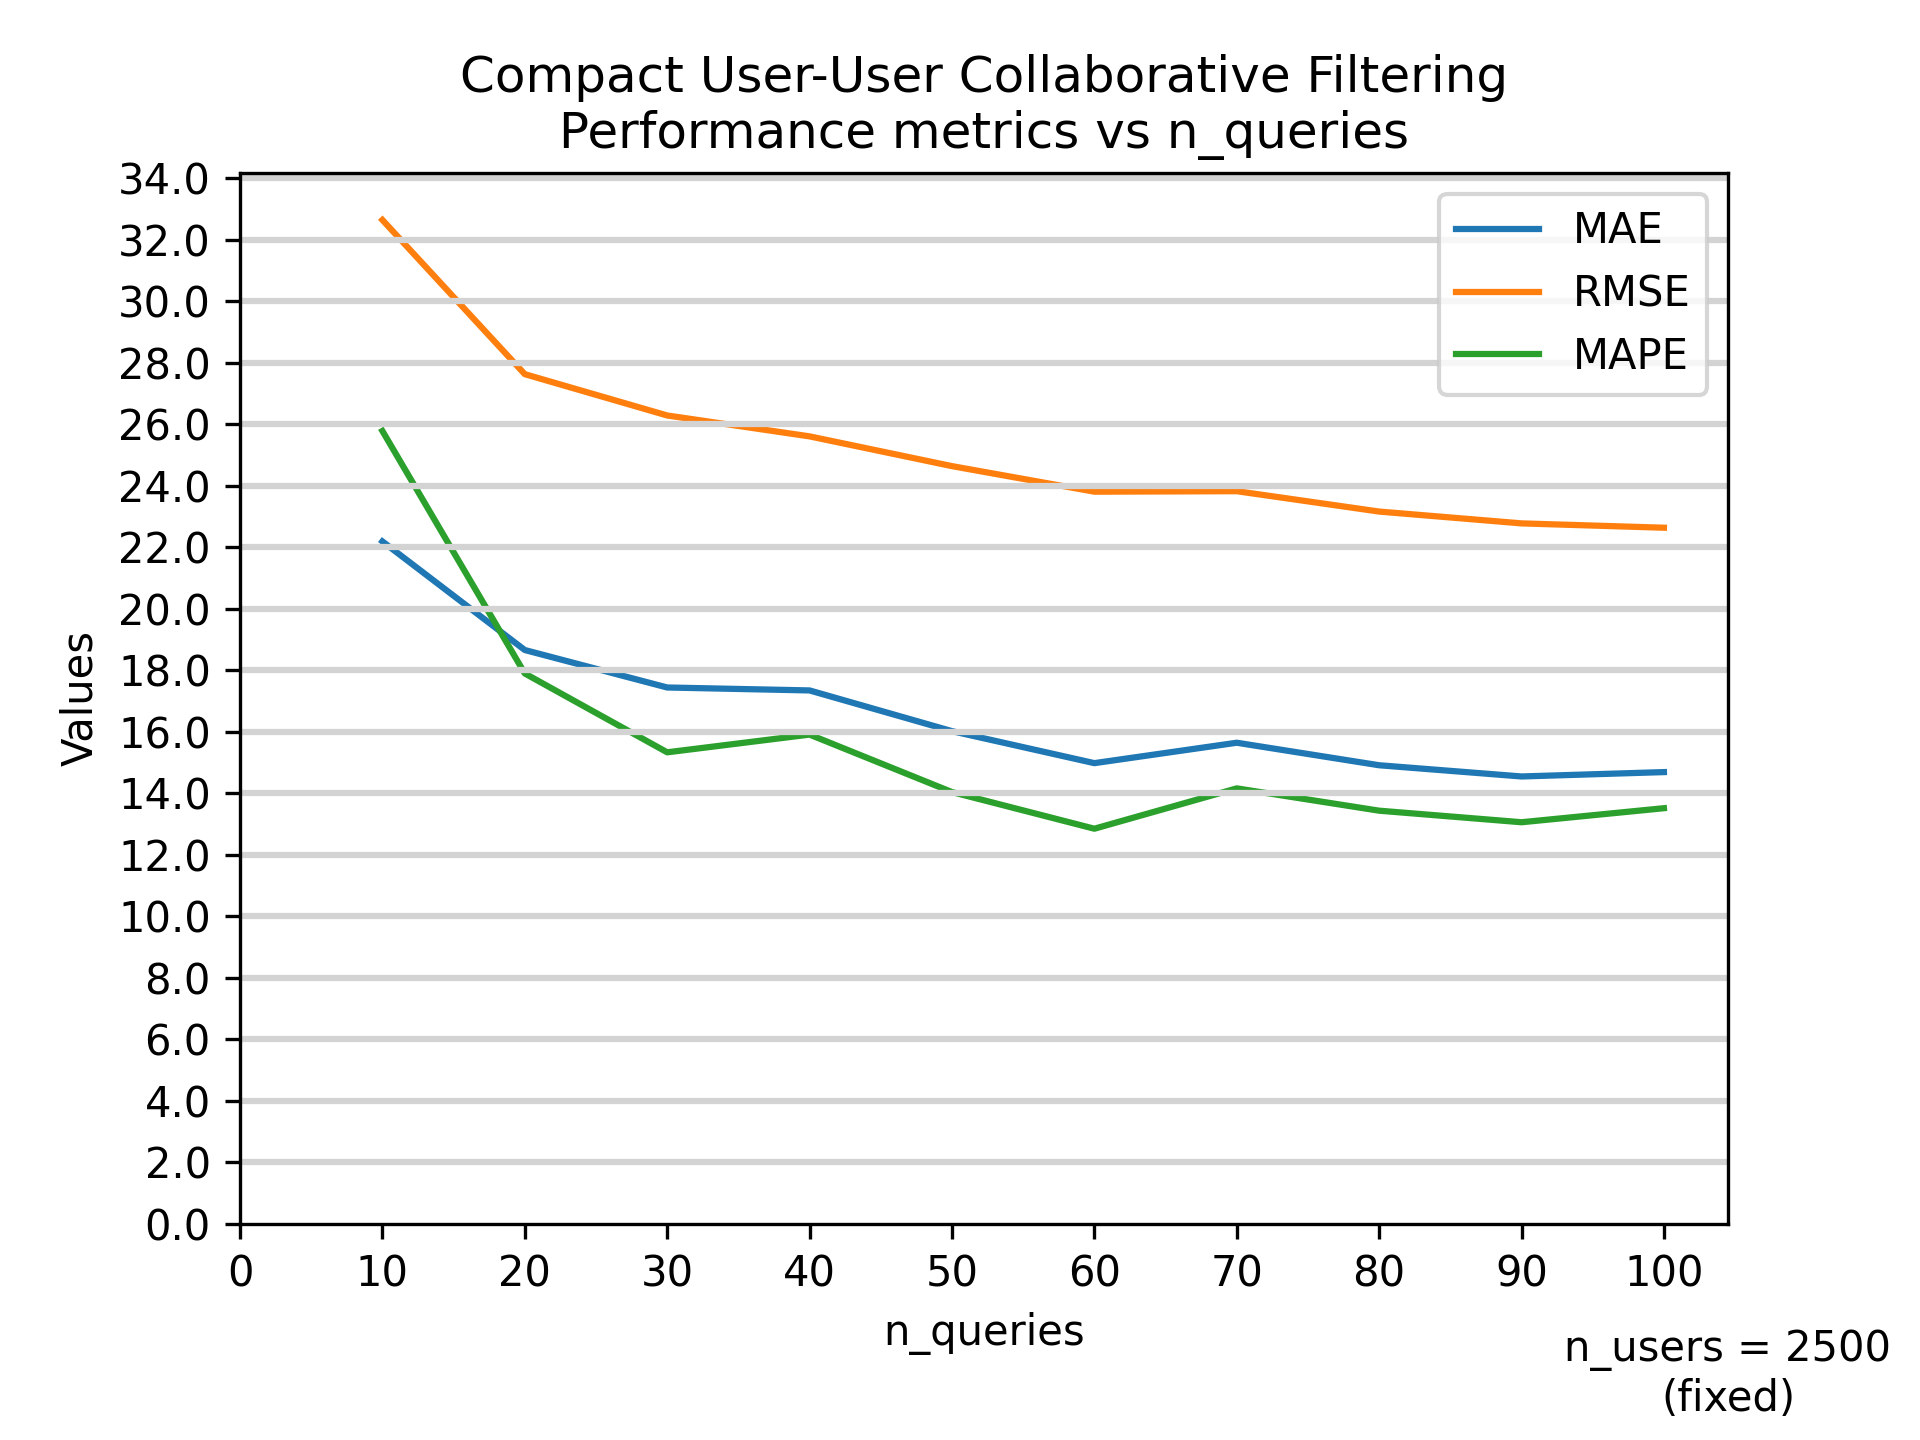
\includegraphics[width=9cm]{Data Mining/images/compact_user_user_queries.png}
\caption{Evaluation metrics of Compact User-User CF, varying number of queries}
\label{fig:Compact User-User CF, varying queries}
\end{figure}


\subsubsection{Expanded Item-Item CF metrics values}

When tested, this component behaves similarly to the previous ones, but the main difference is that it reaches a performance plateau for all three evaluation metrics at a much \textbf{faster} "speed", that is, after only 15 users considered, as shown in Table \ref{tab:expanded Item-Item CF, nitems fixed} and in Figure \ref{fig:Expanded Item-Item CF, varying users} (representing only data considering the first 100 users).


\begin{table}[h!]
    \centering
    \begin{tabular}{ |p{2cm}||p{1.5cm}|p{1.5cm}|p{1.5cm}|  }
         \hline
         \multicolumn{4}{|c|}{Expanded Item-Item CF, n\_items (7669) fixed } \\
         \hline
         \textbf{N\_USERS}& \textbf{MAE} &\textbf{RMSE} &\textbf{MAPE}\\
         \hline
         2 & 7.3249 & 16.2740  & 13.6591\\
         5 & 2.94 & 5.4743  & 5.9994\\
         15 & 2.616  & 4.8884  & 5.6474\\
         50 & 2.6342 & 4.9518 & 5.7490\\
         100 & 2.641  & 4.9109 & 5.7269\\
         200 & 2.6540 & 4.9446 & 5.7057\\
         1250 & 2.7587 & 5.1672 & 5.9894\\
         \textbf{2500} & \textbf{2.7630} & \textbf{5.1779} & \textbf{5.9939}\\
 
         \hline
    \end{tabular}
    \caption{Expanded Item-Item CF, n\_items fixed}
    \label{tab:expanded Item-Item CF, nitems fixed}
\end{table}


\begin{figure}[h!]
\centering
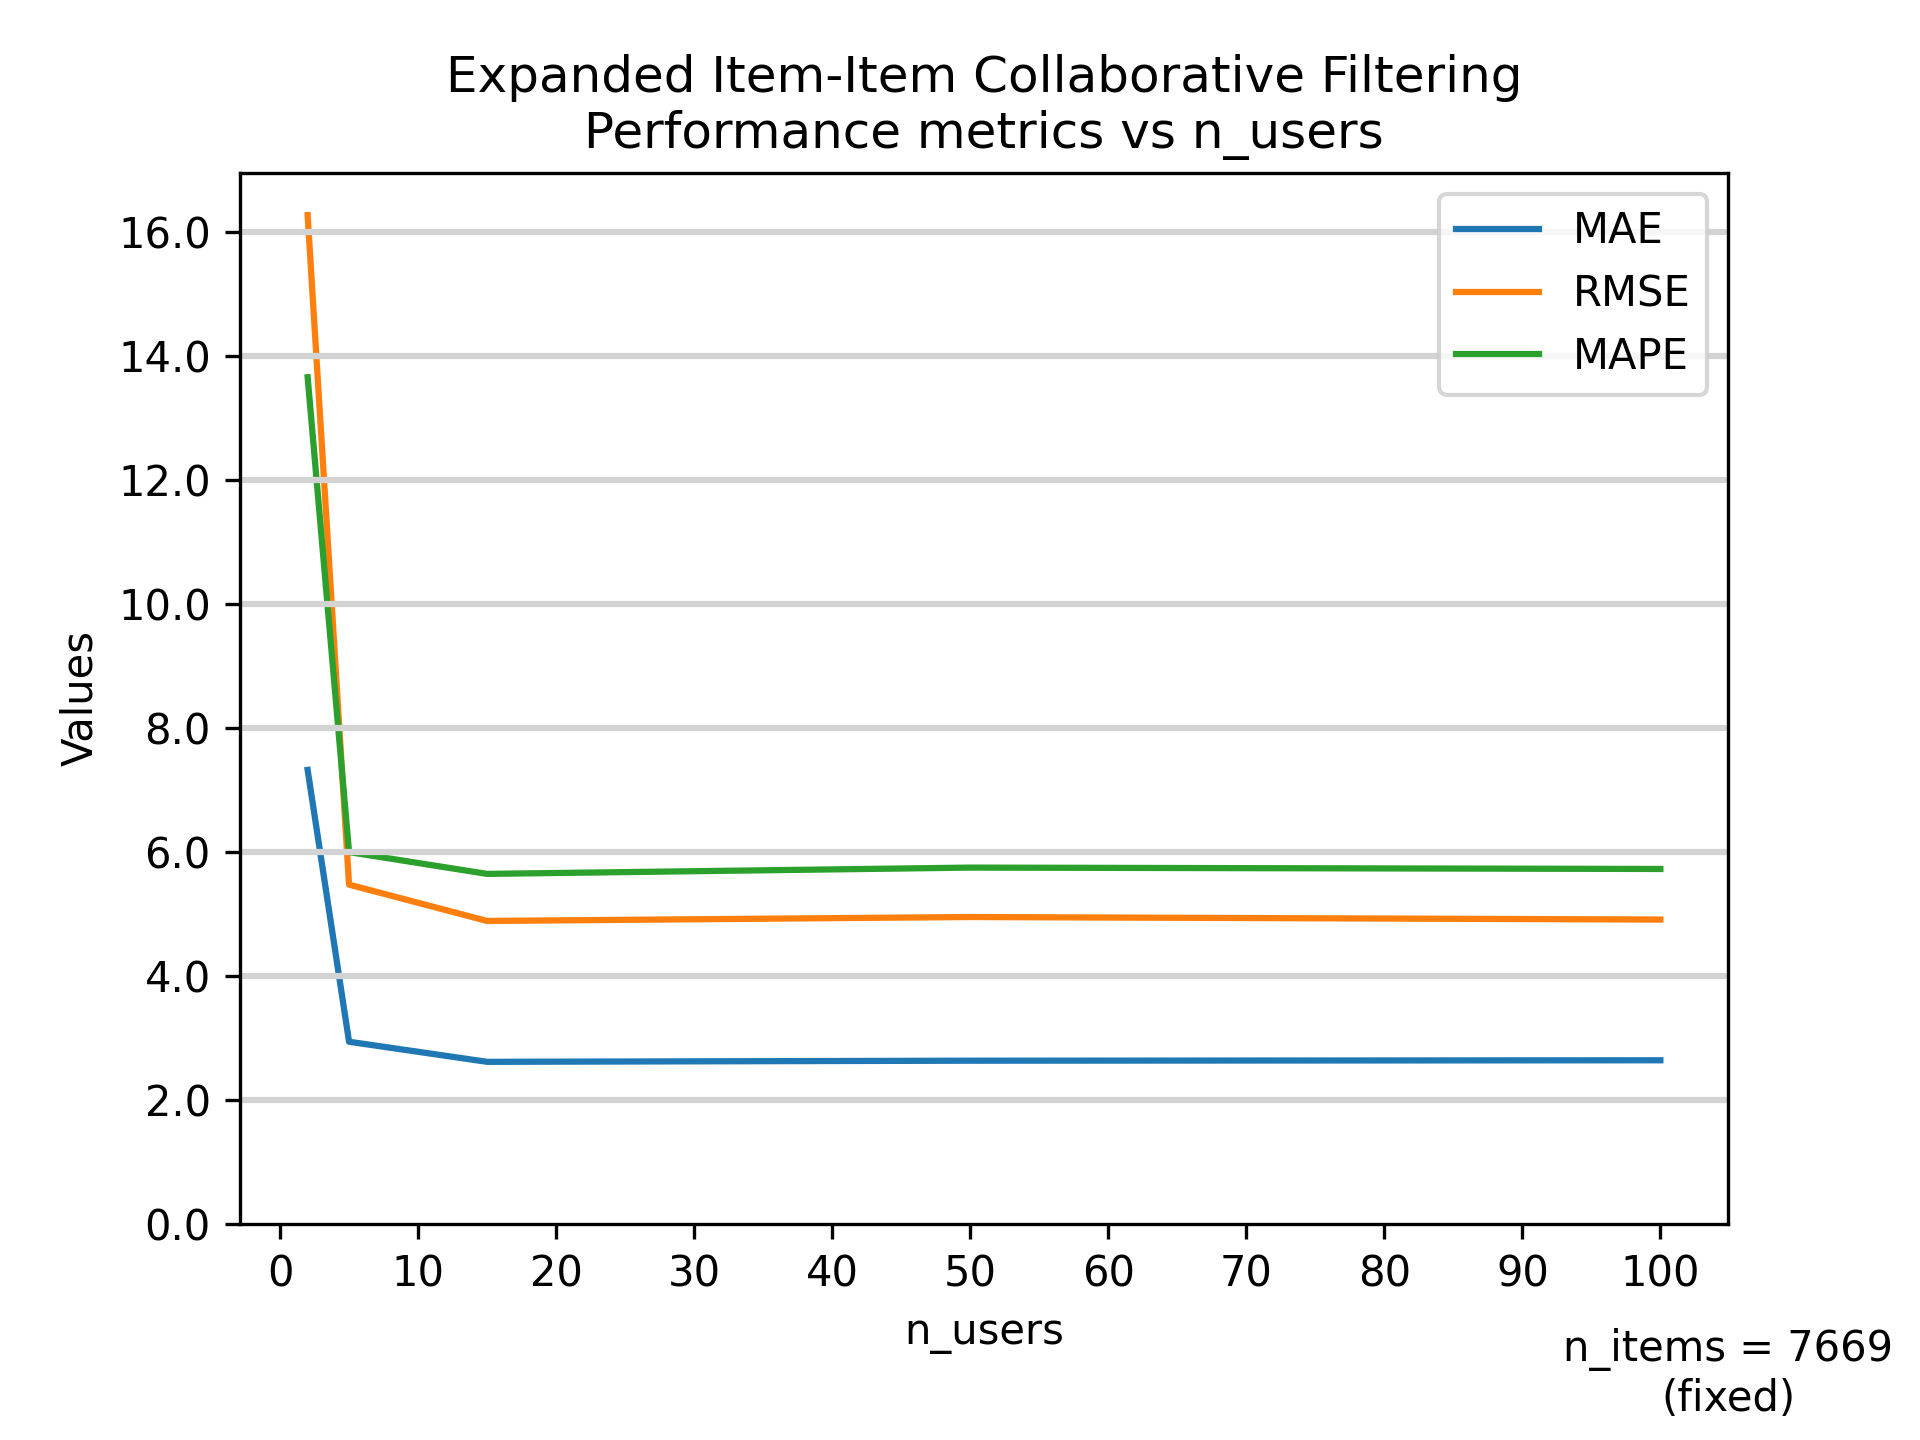
\includegraphics[width=9cm]{Data Mining/images/expanded_item_item_users.png}
\caption{Evaluation metrics of Expanded Item-Item CF, varying number of users}
\label{fig:Expanded Item-Item CF, varying users}
\end{figure}




\subsection{Baseline selection}
\subsubsection{Part A}
\label{sec:baseline-partA}
Among all the approaches that were implemented during the project development, it was chosen as baseline to be used as comparison meter for the PART\_A, the \textbf{Compact} (Standard) \textbf{Item-Item Collaborative Filtering} component described in the Section \ref{sec:compact-item-item-cf-solution}, mainly due to the implementation availability and popularity of that approach in Data Science related works.
\subsubsection{Part B}
Regarding the baseline chosen in order to allow a comparison with the solution described in the subchapter \ref{ch:5.7.2} for the PART\_B, it was decided to expand, as described in the Algorithm \ref{alg:partb_ch4.5.2}, the \textit{Complete Utility Matrix} obtained by running the \textbf{Expanded Item-Item Collaborative Filtering} on the Utility Matrix $U$. The obtained Complete \textit{user-RelationalItem\_utility\_matrix} was used to compute the ratings regarding the new queries.


\subsection{Experimental results accomplished by hybrid solution}
\subsubsection{Part A}
\label{sec:results-hybrid-parta}
To compare the baseline chosen in section \ref{sec:baseline-partA} to the final solution, two main strategies were put in place:  evaluate their ability in correctly \textbf{filling} the Utility Matrix $U$ and, to give the task a more practical meaning, the approaches were also compared in the efficiency in \textbf{finding} the \textit{TOP\_K} queries belonging to the users of the User Set $US$ considered.

Concerning the ability in filling the Utility Matrix $U$, it was actually computed, using both the solution and the baseline method, a \textit{Complete Utility Matrix}, which was then compared to the \textit{Real Complete} one, computed as described in the subsection \ref{ch:5.2}. Referring to the Table \ref{tab:part-a-baseline}, it is possible to see that with the current dataset under consideration (considering N\_QUERIES = 100, N\_USERS = 2500), the proposed solution \textbf{performs slightly better} than the baseline in \textbf{all} of the evaluation metrics proposed.

The configuration parameters for the hybrid solution are:
\begin{itemize}
    \item THRESHOLD\_1 = 200.0
    \item THRESHOLD\_2 = 1000.0
    \item WEIGHT\_1 = 0.75
    \item WEIGHT\_2 = 0.5
    \item WEIGHT\_3 = 0.25
\end{itemize}
    

\begin{table}[h!]
    \centering
    \begin{tabular}{ |p{2cm}||p{1.5cm}|p{1.5cm}|p{1.5cm}|  }
         \hline
         \multicolumn{4}{|c|}{PART A - Utility Matrix: Compact Item-Item CF vs. Hybrid} \\
         \hline
         \textbf{Method}& \textbf{MAE} &\textbf{RMSE} &\textbf{MAPE}\\
         \hline

         \textbf{Baseline} & 3.1420 & 5.7890 & 6.8218\\
         \textbf{Final solution} & \textbf{2.7446} & \textbf{5.1184} & \textbf{5.9671}\\
 
         \hline
    \end{tabular}
    \caption{PART A - Utility Matrix: Baseline vs. Final solution}
    \label{tab:part-a-baseline}
\end{table}


In terms of the second proposed comparison, the \textit{TOP\_K} queries from both the \textit{Complete Utility Matrix} computed by the final solution and the baseline are retrieved. After those query identifiers have been stored in \textbf{two sets} for each user (baseline, solution), they are compared with the actual \textit{TOP\_K} queries set belonging to the \textit{Real Complete Utility Matrix} from the dataset, using the \textbf{Jaccard similarity coefficient} as distance. It should be remarked that the higher the value, the more similar the two sets are.
This distance is calculated considering multiple values of $K$.
The minimum, maximum and mean value of the Jaccard index for each value of $K$ considered are reported in Table \ref{tab:jaccard}.

A \textbf{Dot-Box plot}, represented in Figure \ref{fig:jaccard-topk-parta}, is used to visualize the distribution of the gathered data, showing the median (middle line in the box), 25th quartile (lower edge of the box), 75th quartile (higher edge of the box), and the outliers. The dots, in addition, give a sense of how many data points lie within each group.  
As we can see in the figure, for the first 5 values of K, the lowest, median and highest values of the Jaccard index are the same for both the baseline and the solution. 
This suggests that there is basically \textbf{no advantage} in using a hybrid approach with respect to a standard one, for low K values, i.e., small sets of highest rated queries. 
Starting from the value K = 10, median, 25th quartile and 75th quartile values related to the solution are \textbf{higher}, as it can be seen by the middle line, lower and higher edge of the boxes.
It could be also noted that, for all the values of K considered, as Table \ref{tab:jaccard} shows, the mean of the Jaccard similarity coefficient is always \textbf{slightly higher} for the solution.


\begin{table}[]
\begin{tabular}{l|lll|}
\cline{2-4}
                                          & \multicolumn{3}{l|}{Jaccard similarity coefficient, versus real dataset}    \\ \hline
\multicolumn{1}{|l|}{\textbf{TOP\_K}}              & \multicolumn{1}{l|}{\textbf{Min}}       & \multicolumn{1}{l|}{\textbf{Max}}       & \textbf{Mean}      \\ \hline
\multicolumn{1}{|l|}{\multirow{2}{*}{1}}  & \multicolumn{1}{l|}{C: 0.0}    & \multicolumn{1}{l|}{C: 1.0}    & C: 0.3176 \\ \cline{2-4} 
\multicolumn{1}{|l|}{}                    & \multicolumn{1}{l|}{H: 0.0}    & \multicolumn{1}{l|}{H: 1.0}    & H: 0.3296 \\ \hline
\multicolumn{1}{|l|}{\multirow{2}{*}{2}}  & \multicolumn{1}{l|}{C: 0.0}    & \multicolumn{1}{l|}{C: 1.0}    & C: 0.2621 \\ \cline{2-4} 
\multicolumn{1}{|l|}{}                    & \multicolumn{1}{l|}{H: 0.0}    & \multicolumn{1}{l|}{H: 1.0}    & H: 0.2814 \\ \hline
\multicolumn{1}{|l|}{\multirow{2}{*}{3}}  & \multicolumn{1}{l|}{C: 0.0}    & \multicolumn{1}{l|}{C: 1.0}    & C: 0.2504 \\ \cline{2-4} 
\multicolumn{1}{|l|}{}                    & \multicolumn{1}{l|}{H: 0.0}    & \multicolumn{1}{l|}{H: 1.0}    & H: 0.2753 \\ \hline
\multicolumn{1}{|l|}{\multirow{2}{*}{4}}  & \multicolumn{1}{l|}{C: 0.0}    & \multicolumn{1}{l|}{C: 1.0}    & C: 0.2529 \\ \cline{2-4} 
\multicolumn{1}{|l|}{}                    & \multicolumn{1}{l|}{H: 0.0}    & \multicolumn{1}{l|}{H: 1.0}    & H: 0.2786 \\ \hline
\multicolumn{1}{|l|}{\multirow{2}{*}{5}}  & \multicolumn{1}{l|}{C: 0.0}    & \multicolumn{1}{l|}{C: 1.0}    & C: 0.2606 \\ \cline{2-4} 
\multicolumn{1}{|l|}{}                    & \multicolumn{1}{l|}{H: 0.0}    & \multicolumn{1}{l|}{H: 1.0}    & H: 0.2862 \\ \hline
\multicolumn{1}{|l|}{\multirow{2}{*}{10}} & \multicolumn{1}{l|}{C: 0.0}    & \multicolumn{1}{l|}{C: 0.8181} & C: 0.2821 \\ \cline{2-4} 
\multicolumn{1}{|l|}{}                    & \multicolumn{1}{l|}{H: 0.0}    & \multicolumn{1}{l|}{H: 0.8181} & H: 0.3115 \\ \hline
\multicolumn{1}{|l|}{\multirow{2}{*}{15}} & \multicolumn{1}{l|}{C: 0.0}    & \multicolumn{1}{l|}{C: 0.7647} & C: 0.3098 \\ \cline{2-4} 
\multicolumn{1}{|l|}{}                    & \multicolumn{1}{l|}{H: 0.0}    & \multicolumn{1}{l|}{H: 0.875}  & H: 0.3373 \\ \hline
\multicolumn{1}{|l|}{\multirow{2}{*}{20}} & \multicolumn{1}{l|}{C: 0.0256} & \multicolumn{1}{l|}{C: 0.7391} & C: 0.3436 \\ \cline{2-4} 
\multicolumn{1}{|l|}{}                    & \multicolumn{1}{l|}{H: 0.0526} & \multicolumn{1}{l|}{H: 0.8181} & H: 0.3696 \\ \hline
\multicolumn{1}{|l|}{\multirow{2}{*}{30}} & \multicolumn{1}{l|}{C: 0.1538} & \multicolumn{1}{l|}{C: 0.8181} & C: 0.4309 \\ \cline{2-4} 
\multicolumn{1}{|l|}{}                    & \multicolumn{1}{l|}{H: 0.1320} & \multicolumn{1}{l|}{H: 0.7647} & H: 0.4576 \\ \hline
\end{tabular}
\caption{PART A - TOP-K queries: Baseline (C) vs. Final Solution (H)}
\label{tab:jaccard}
\end{table}



\begin{figure}[h!]
\centering
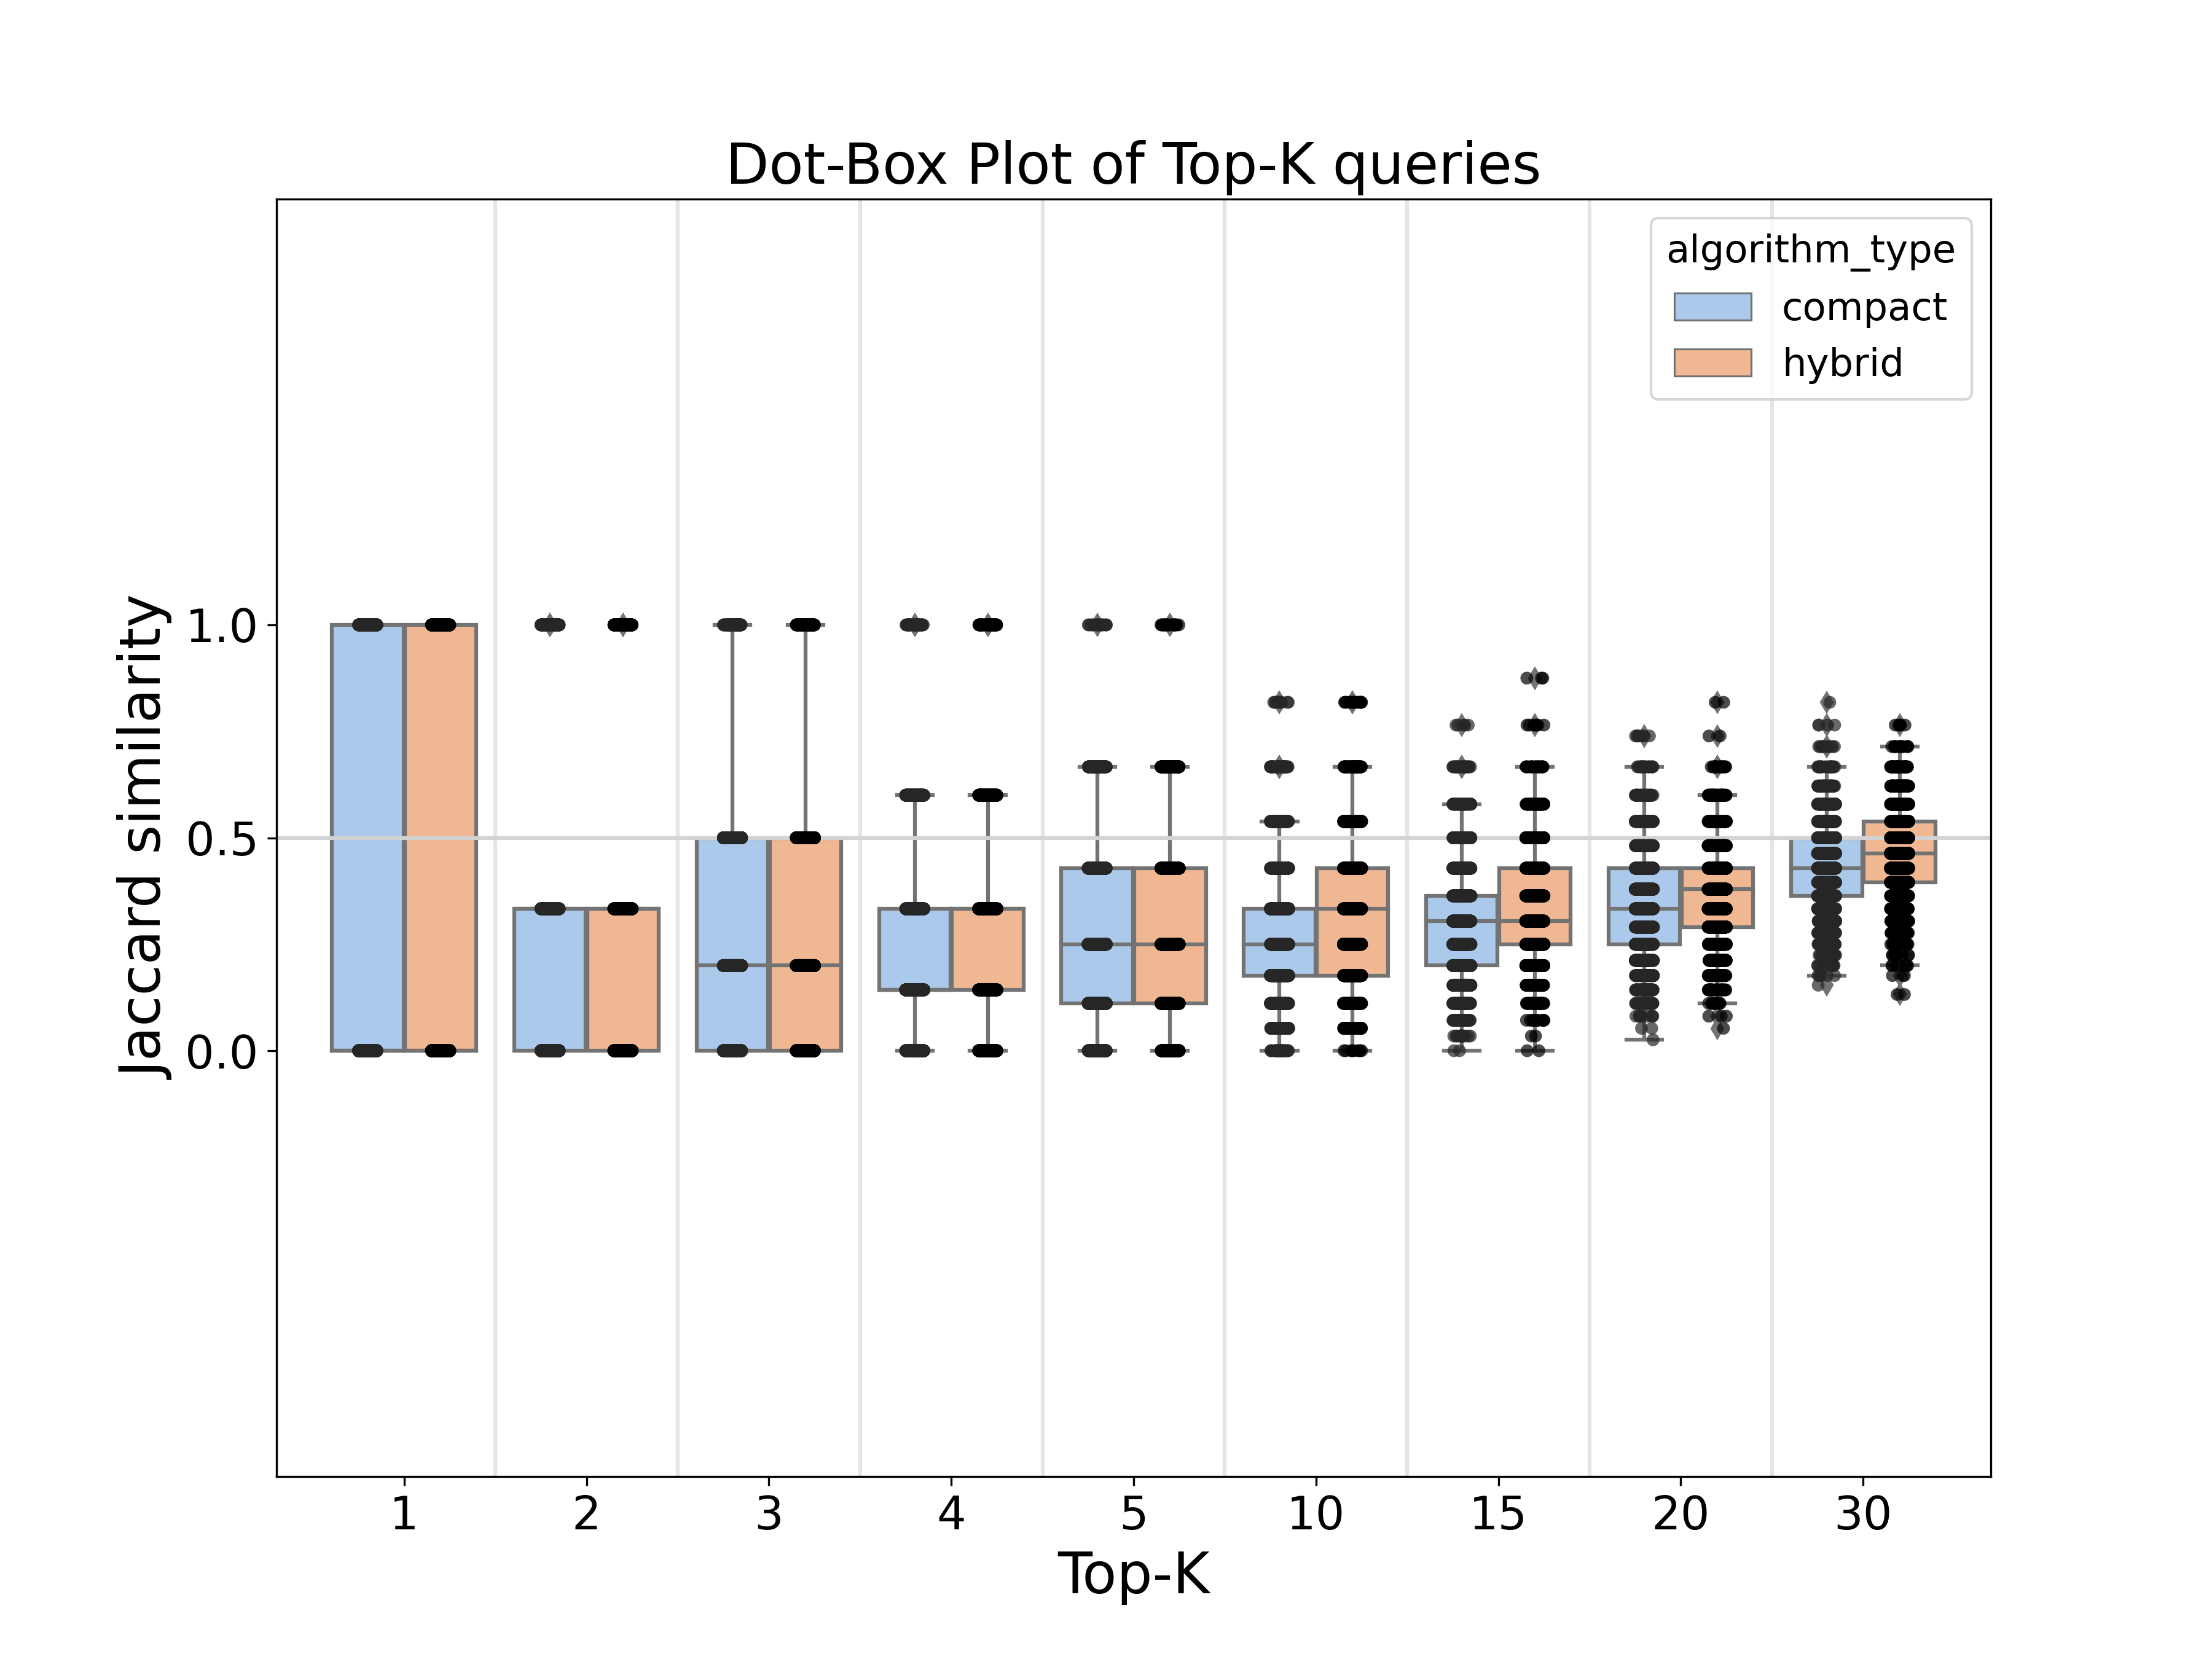
\includegraphics[width=9cm]{Data Mining/images/jaccard_part_a.png}
\caption{PART A - Jaccard similarity for the Top-K queries sets}
\label{fig:jaccard-topk-parta}
\end{figure}




\subsubsection{Part B} \label{ch:5.7.2}
Regarding the comparison of the second baseline chosen with our solution, a similar approach to the one described in the subsection \ref{sec:results-hybrid-parta} was followed. So, given some new and unseen queries, there were built 3 new utility matrices:
\begin{itemize}
    \item A \textit{New Real Complete Utility Matrix}, obtained by comparing the results of each new query with the existing users profiles as described in the Algorithm \ref{alg:users-queries score computation}.
    \item A \textit{Baseline Complete Utility Matrix}, obtained by computing a prediction for every user-query combination as described in the Algorithm \ref{alg:partb-ch4.5.1}. The intermediate \textit{Baseline User-Relational Item Utility Matrix} was the same obtained by the expansion described in the subchapter \ref{sub:expansion}  and the users and queries taken into account during the compression were the same of the \textit{New Real Complete Utility Matrix}.
    \item Another \textit{Hybrid Complete Utility Matrix} built by expanding and then compressing the Utility Matrix computed by our solution described in the subchapter \ref{sec:results-hybrid-parta}. The expansion was done considering the definition of the original Utility Matrix $U$ being part of our problem statement while the compression was done considering the new queries proposed during the PART\_B, as described in the subchapter \ref{ch:4.2.3}.
\end{itemize}

Once obtained those three Utility Matrices, the \textit{New Real Complete Utility Matrix} is compared with the baseline one and with the hybrid one (representing our solution), using the three evaluation metrics described in the subsection \ref{sec:evaluation-metrics}. The results are shown in Table \ref{tab:part-b-baseline} where it can be seen that the final solution has performed \textbf{slightly better} in 2 out of 3 evaluation metrics. However, the values gathered at this stage are all very similar to one another.



As done for the PART\_A, in order to evaluate the solution in a more practical term, the \textit{TOP\_K} queries from both the Complete Utility Matrix computed by the final solution and from baseline are retrieved. After those query identifiers have been stored in two sets for each user (baseline, solution), they are compared with the actual \textit{TOP\_K} queries set belonging to the Real Complete Utility Matrix that has been created for PART\_B, using the Jaccard similarity coefficient as distance.

As for PART\_A, the minimum, maximum and mean value of the Jaccard index for each value of K considered are reported in Table \ref{tab:jaccardB}.
Another \textbf{Dot-Box plot}, represented in Figure \ref{fig:jaccard-topk-partb}, is used to visualize the distribution of the data.
Looking at the latter, the results obtained are \textbf{nearly identical} for each value of k considered. One thing to note is that in the case of maximum k tested (25) the 25th quartile associated with the hybrid method has a slightly higher jaccard index than the 25th quartile associated with the expanded method.


\begin{table}[h!]
    \centering
    \begin{tabular}{ |p{2cm}||p{1.5cm}|p{1.5cm}|p{1.5cm}|  }
         \hline
         \multicolumn{4}{|c|}{PART B - Utility Matrix: Expanded Item-Item CF vs. Hybrid} \\
         \hline
         \textbf{Method}& \textbf{MAE} &\textbf{RMSE} &\textbf{MAPE}\\
         \hline

         \textbf{Baseline} & 4.0507  & 6.1362  &  \textbf{8.6332}\\
         \textbf{Final solution} & \textbf{4.040864} & \textbf{6.1086} & 8.6342 \\
 
         \hline
    \end{tabular}
    \caption{PART B - Utility Matrix: Baseline vs. Final solution}
    \label{tab:part-b-baseline}
\end{table}


\begin{table}[]
\begin{tabular}{l|lll|}
\cline{2-4}
                                          & \multicolumn{3}{l|}{Jaccard similarity coefficient, versus real dataset}    \\ \hline
\multicolumn{1}{|l|}{\textbf{TOP\_K}}              & \multicolumn{1}{l|}{\textbf{Min}}       & \multicolumn{1}{l|}{\textbf{Max}}       & \textbf{Mean}      \\ \hline
\multicolumn{1}{|l|}{\multirow{2}{*}{1}}  & \multicolumn{1}{l|}{E: 0.0}    & \multicolumn{1}{l|}{E: 1.0}    & E: 0.1112 \\ \cline{2-4} 
\multicolumn{1}{|l|}{}                    & \multicolumn{1}{l|}{H: 0.0}    & \multicolumn{1}{l|}{H: 1.0}    & H: 0.1148 \\ \hline
\multicolumn{1}{|l|}{\multirow{2}{*}{2}}  & \multicolumn{1}{l|}{E: 0.0}    & \multicolumn{1}{l|}{E: 1.0}    & E: 0.1497 \\ \cline{2-4} 
\multicolumn{1}{|l|}{}                    & \multicolumn{1}{l|}{H: 0.0}    & \multicolumn{1}{l|}{H: 1.0}    & H: 0.1544 \\ \hline
\multicolumn{1}{|l|}{\multirow{2}{*}{3}}  & \multicolumn{1}{l|}{E: 0.0}    & \multicolumn{1}{l|}{E: 1.0}    & E: 0.1725 \\ \cline{2-4} 
\multicolumn{1}{|l|}{}                    & \multicolumn{1}{l|}{H: 0.0}    & \multicolumn{1}{l|}{H: 1.0}    & H: 0.1781 \\ \hline
\multicolumn{1}{|l|}{\multirow{2}{*}{4}}  & \multicolumn{1}{l|}{E: 0.0}    & \multicolumn{1}{l|}{E: 1.0}    & E: 0.1935 \\ \cline{2-4} 
\multicolumn{1}{|l|}{}                    & \multicolumn{1}{l|}{H: 0.0}    & \multicolumn{1}{l|}{H: 1.0}    & H: 0.1998 \\ \hline
\multicolumn{1}{|l|}{\multirow{2}{*}{5}}  & \multicolumn{1}{l|}{E: 0.0}    & \multicolumn{1}{l|}{E: 1.0}    & E: 0.2083 \\ \cline{2-4} 
\multicolumn{1}{|l|}{}                    & \multicolumn{1}{l|}{H: 0.0}    & \multicolumn{1}{l|}{H: 1.0}    & H: 0.2120 \\ \hline
\multicolumn{1}{|l|}{\multirow{2}{*}{10}} & \multicolumn{1}{l|}{E: 0.0}    & \multicolumn{1}{l|}{E: 0.8181} & E: 0.2722 \\ \cline{2-4} 
\multicolumn{1}{|l|}{}                    & \multicolumn{1}{l|}{H: 0.0}    & \multicolumn{1}{l|}{H: 0.8181} & H: 0.2802 \\ \hline
\multicolumn{1}{|l|}{\multirow{2}{*}{15}} & \multicolumn{1}{l|}{E: 0.0714}    & \multicolumn{1}{l|}{E: 0.7647} & E: 0.3596 \\ \cline{2-4} 
\multicolumn{1}{|l|}{}                    & \multicolumn{1}{l|}{H: 0.0714}    & \multicolumn{1}{l|}{H: 0.7647}  & H: 0.3671 \\ \hline
\multicolumn{1}{|l|}{\multirow{2}{*}{20}} & \multicolumn{1}{l|}{E: 0.3513} & \multicolumn{1}{l|}{E: 0.9230} & E: 0.5917 \\ \cline{2-4} 
\multicolumn{1}{|l|}{}                    & \multicolumn{1}{l|}{H: 0.3513} & \multicolumn{1}{l|}{H: 0.8518} & H: 0.5972 \\ \hline
\end{tabular}
\caption{PART B - TOP-K queries: Baseline (E) vs. Final Solution (H)}
\label{tab:jaccardB}
\end{table}

\begin{figure}[h!]
\centering
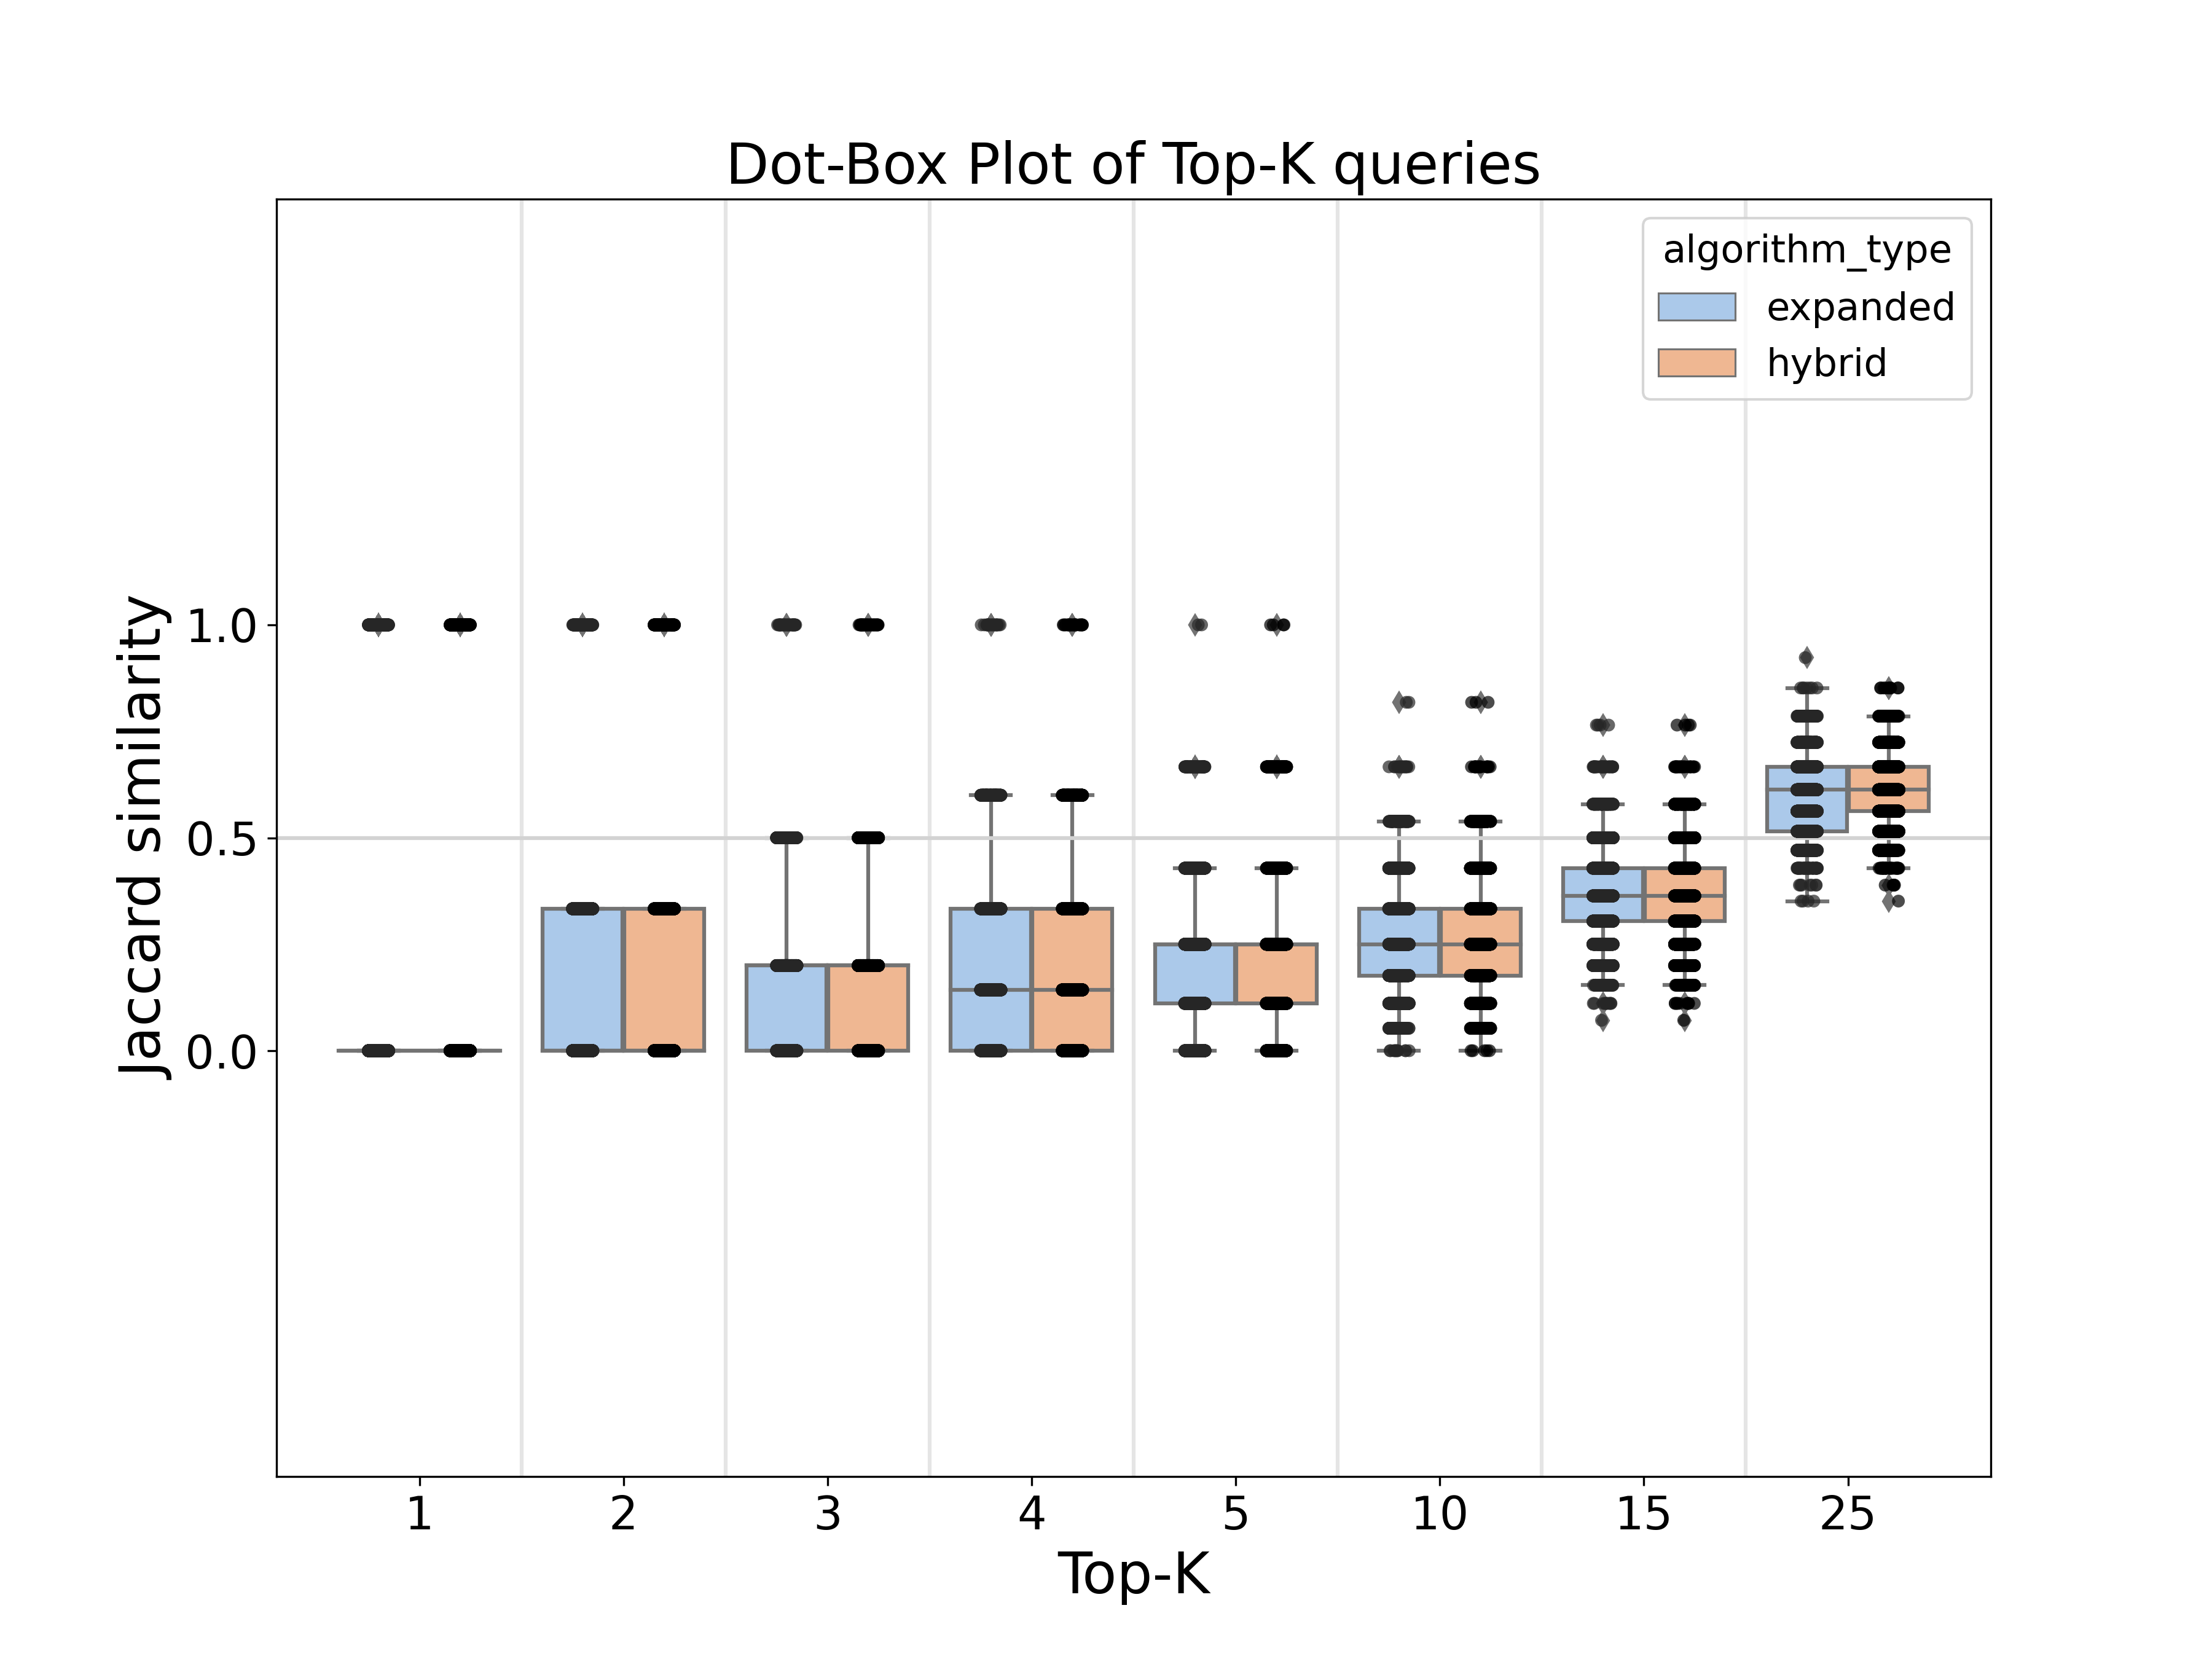
\includegraphics[width=9cm]{Data Mining/images/jaccard_part_b.png}
\caption{PART B - Jaccard similarity for the Top-K queries sets}
\label{fig:jaccard-topk-partb}
\end{figure}




\section{Conclusion}
\label{sec:conclusion}

To conclude, the main underlying philosophy followed during the development of all the approaches tried was related in finding a valid solution through iterations, each of which was capable of improving the previously best one found. This process resulted in the discovery of a solution composed of a \textbf{hybrid recommendation system} leveraging a linear combination of \textbf{Expanded-Item-Item Collaborative Filtering} and \textbf{Compact Item-Item Collaborative Filtering} based on \textbf{query result cardinality}. There was also the intent of the development of a modular solution. The use of shared components and algorithms between the various described sub-tasks demonstrates this.

The proposed solution was able, at the expense of slower performance, to \textbf{slightly improve} in correctness all the other solutions with standard implementations or developed from scratch. The improvement was most noticeable during evaluations in which the \textit{Utility Matrix} filled by the proposed solution for both PART A and PART B was compared, using the \textbf{three evaluation metrics}, with the actual \textit{Real Complete Utility Matrix} generated during the dataset construction. In terms of the evaluation of the \textit{TOP\_K} queries of each user computed by the proposed solution, performed using the \textbf{Jaccard Similarity}, there was almost \textbf{no significant advantage} in using the hybrid solution over the baselines.

In conclusion, the project's development was useful in understanding that in order to create a successful recommendation system, it is often necessary to rely on multiple approaches to achieve a better final outcome. There is definitely \textbf{room for improvement}, both in terms of the analysis of smart combinations of components and larger-scale testing.










%%
%% The acknowledgments section is defined using the "acks" environment
%% (and NOT an unnumbered section). This ensures the proper
%% identification of the section in the article metadata, and the
%% consistent spelling of the heading.

%%
%% The next two lines define the bibliography style to be used, and
%% the bibliography file.
\bibliographystyle{ACM-Reference-Format}
\bibliography{bibliography}

%%
%% If your work has an appendix, this is the place to put it.
\appendix

\end{document}
\endinput
%%
%% End of file `sample-sigconf.tex'.


